\documentclass[12pt]{article}


\newcommand{\GroupId}{CC09-7}
\newcommand{\assignment}{project-security}

\NeedsTeXFormat{LaTeX2e}
\usepackage[osf]{mathpazo}
\usepackage[svgnames]{xcolor}
\usepackage[T1]{fontenc}
\usepackage{amsmath,amsthm,amsfonts,amssymb,mathtools}
\usepackage{hyperref,url}
\usepackage{float}
\usepackage[margin=2.7cm,a4paper]{geometry}
\usepackage{tasks}
\usepackage{xstring}
\usepackage[tikz]{mdframed}
\usepackage{environ}
\usepackage{subcaption}
\usepackage{etoolbox}
\usepackage{fourier-orns}
\usepackage{kvoptions}
\usepackage[]{units}
\usepackage{url}%
%\usepackage[normal]{subfigure}

% math config

\DeclarePairedDelimiter\ceil{\lceil}{\rceil}
\DeclarePairedDelimiter\abs{\lvert}{\rvert}
\DeclarePairedDelimiter\set{\{}{\}}


% headers

\usepackage{fancyhdr}
\addtolength{\headheight}{2.5pt}
\pagestyle{fancy}
\fancyhead{} 
\fancyhead[L]{\sc info2222} % Replace with comp2123 or comp2823
\renewcommand{\headrulewidth}{0.75pt}

% update these headers
\fancyhead[C]{\sc Group Id: \GroupId}
\fancyhead[R]{Assignment \assignment}

\begin{document}

\section{Introduction}

This project is to implement a messaging app for encrypted communication. Based on the given template, we have enabled secure user registration, login, friend requests, and encrypted chats with friends. During the use of the app, we fully ensure the security of the users' information, effectively preventing the potential attacks such as DDoS and man-in-the-middle. Based on the specific scoring criteria , we have done a detailed related report below with screenshots of code and web pages.

\section{Approach explanation}
    \subsection*{Part: Basic Functionality Requirements:}
        \subsubsection*{1} When a user attempts to log in, the frontend initially hashes the user's inputted password using SHA-256, as shown in figure \ref{Hashed Password in frontend}. Then, the username and hashed password are sent to the server. The server checks if the user exists; if not, an error message is displayed, as shown in figure \ref{No such user}. If the user exists, the server hashes the received hashed password again using a salt stored in the database, and then compares this double-hashed password with the hash value stored in the database. If they match, the login is successful, and the user is redirected to the home page, as shown in \ref{login successful}. If they do not match, an error message is displayed, as shown in figure \ref{password doesn't match}.


        When users sign up, to prevent XSS attacks, we have imposed restrictions on the length of usernames and passwords, as well as on the characters that can be used, as shown in Figure \ref{signup xss}.

        \begin{figure}[H]
            \centering
            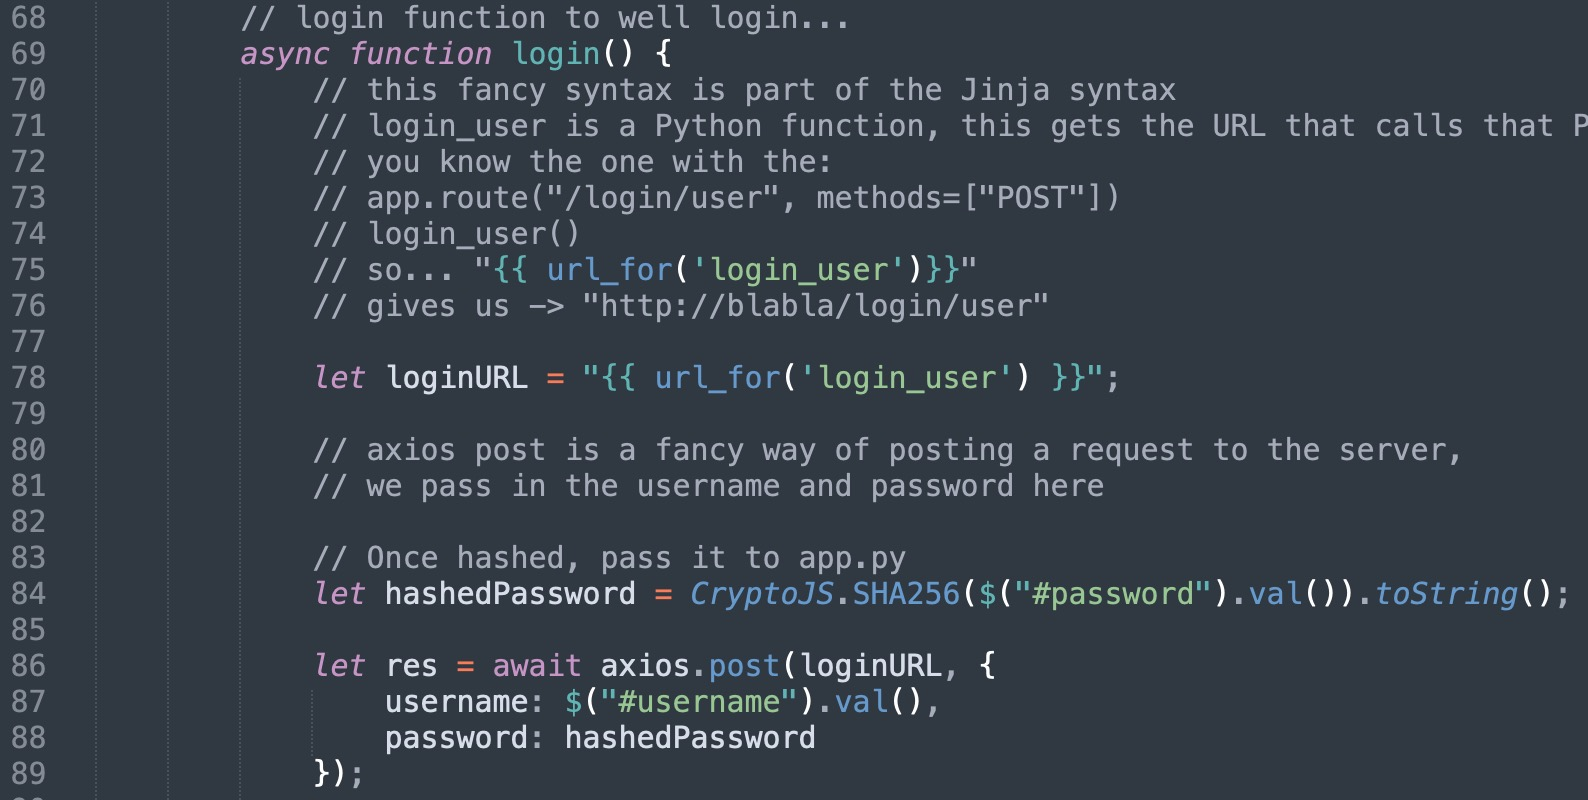
\includegraphics[width=0.8\textwidth]{graphs/front_login_hashed.jpg}
            \caption{Hashed Password in frontend}
            \label{Hashed Password in frontend}
        \end{figure}

        \begin{figure}[H]
            \centering
            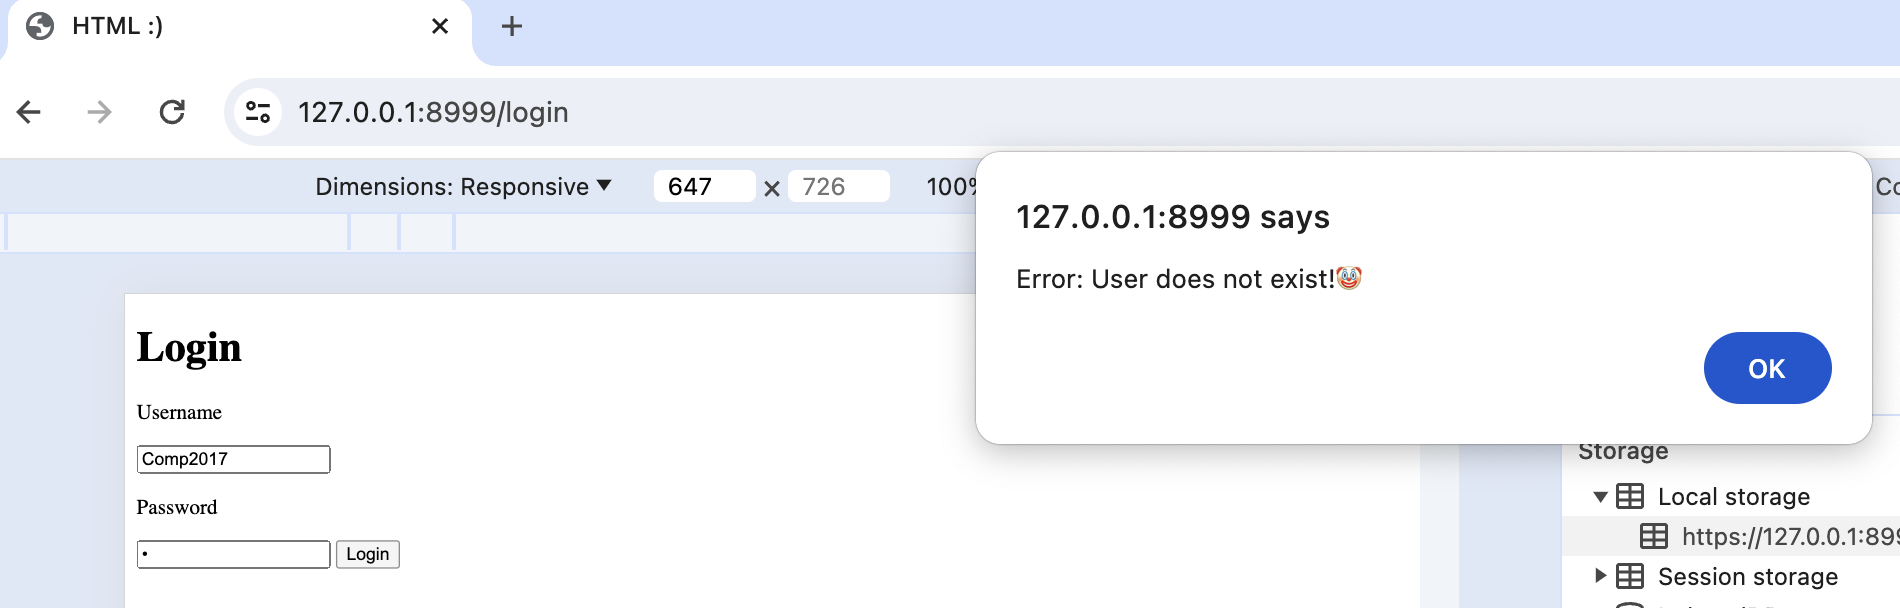
\includegraphics[width=0.8\textwidth]{graphs/no_such_user_login.jpg}
            \caption{No such user}
            \label{No such user}
        \end{figure}

        \begin{figure}[H]
            \centering
            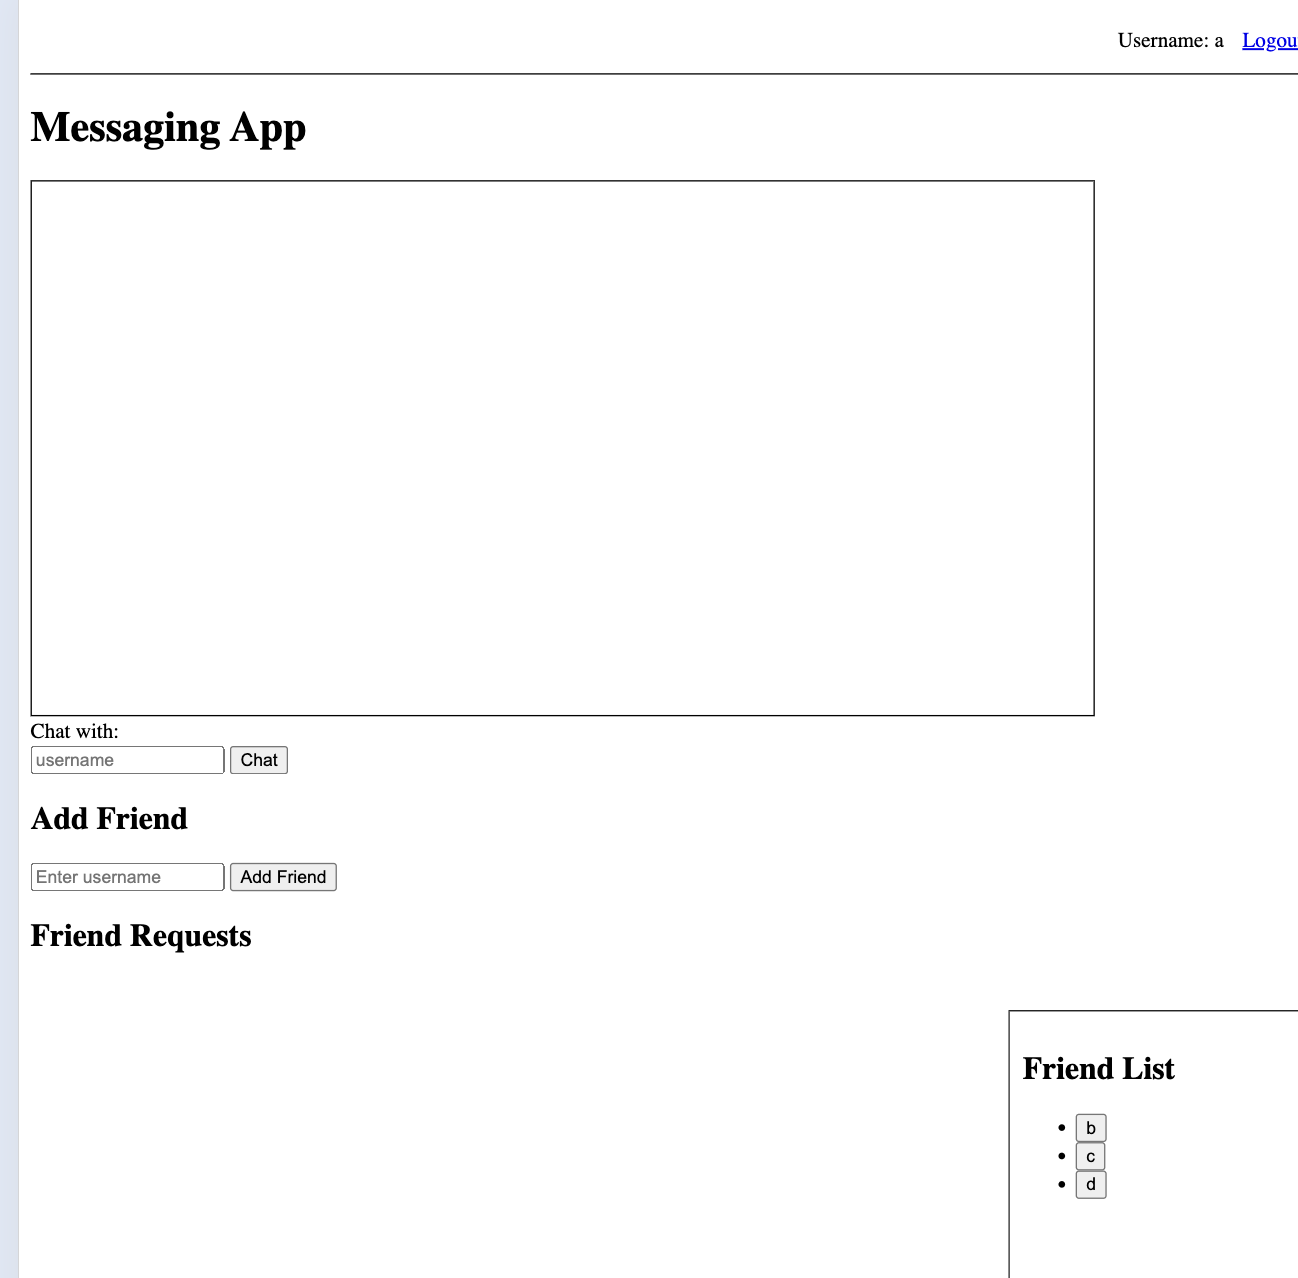
\includegraphics[width=0.8\textwidth]{graphs/login_successful.png}
            \caption{login successful}
            \label{login successful}
        \end{figure}

        \begin{figure}[H]
            \centering
            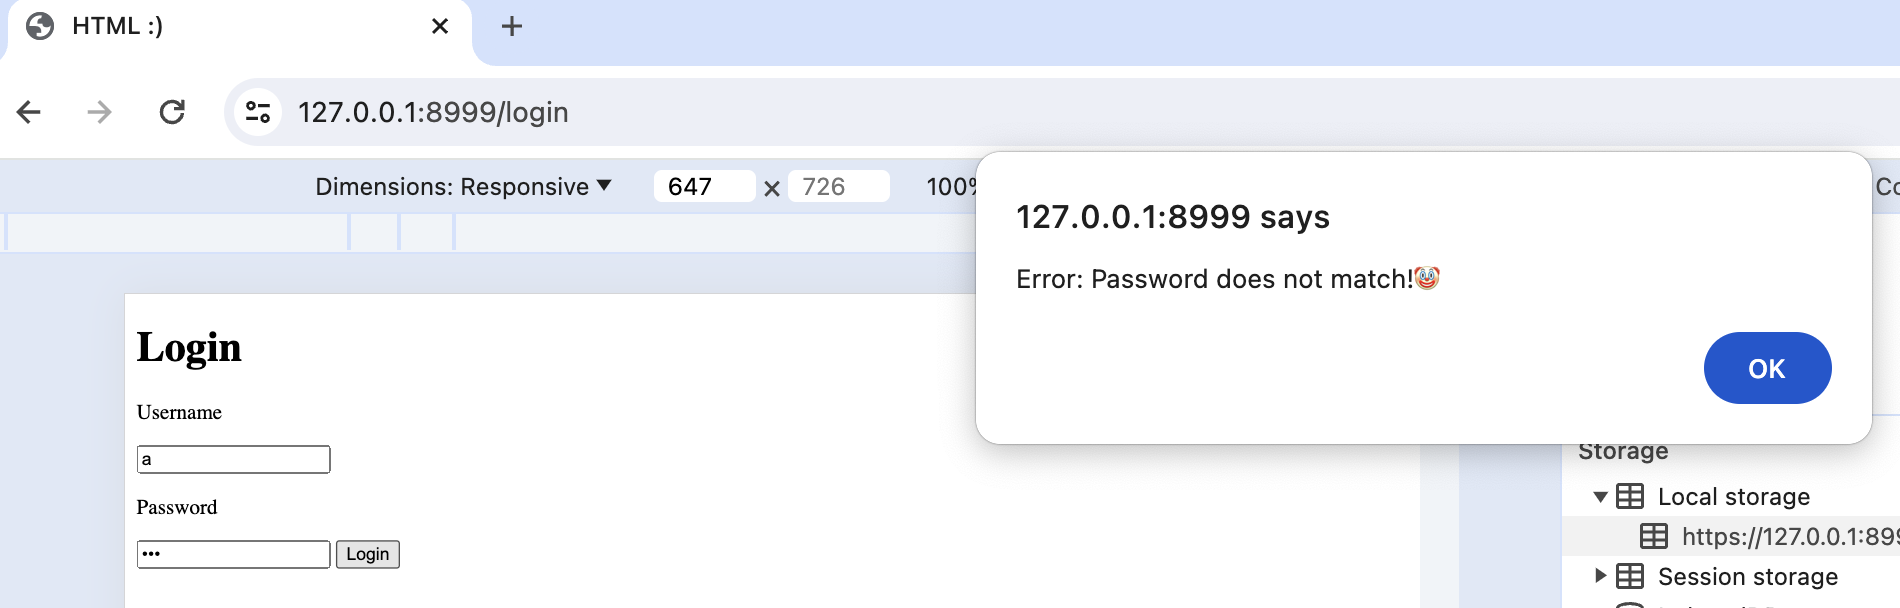
\includegraphics[width=0.8\textwidth]{graphs/passwd_does_not_match.png}
            \caption{password doesn't match}
            \label{password doesn't match}
        \end{figure}

        \begin{figure}[H]
            \centering
            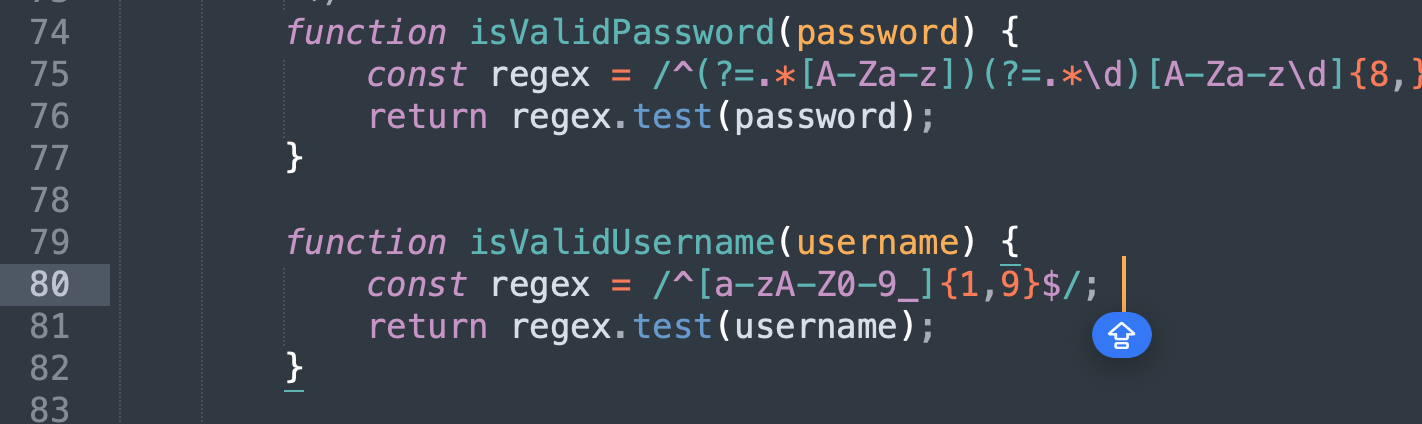
\includegraphics[width=0.8\textwidth]{graphs/sign_up_xss.jpg}
            \caption{signup.jinja}
            \label{signup xss}
        \end{figure}

        \subsubsection*{2} Once user logs in successfully, a dynamic friend list can be shown bottom right the webpage. It displays all the users who this user is friend with as buttons. By clicking on the bottoms, the user can join in the chat room and chat with the friend. In order to implement this feature, we designed a class called friendship (shown in Figure \ref{friendshipClass}) , then we use a function called get friends for user, to get all the users who this user if friend with.(shown in Figure \ref{getfriends}) . Then we use a function called fetchfriends in the frontend to display all the friends as buttons. Once clicking the bottom, it will trigger join room function, which allows user to chat with friends(shown in Figure \ref{fetchfriends}).

        \begin{figure}[H]
            \centering
            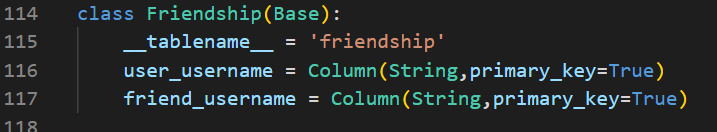
\includegraphics[width=0.8\textwidth]{zzrgraphs/models_friendship.png}
            \caption{models.py define a class called friendship}
            \label{friendshipClass}
        \end{figure}

        \begin{figure}[H]
                \centering
                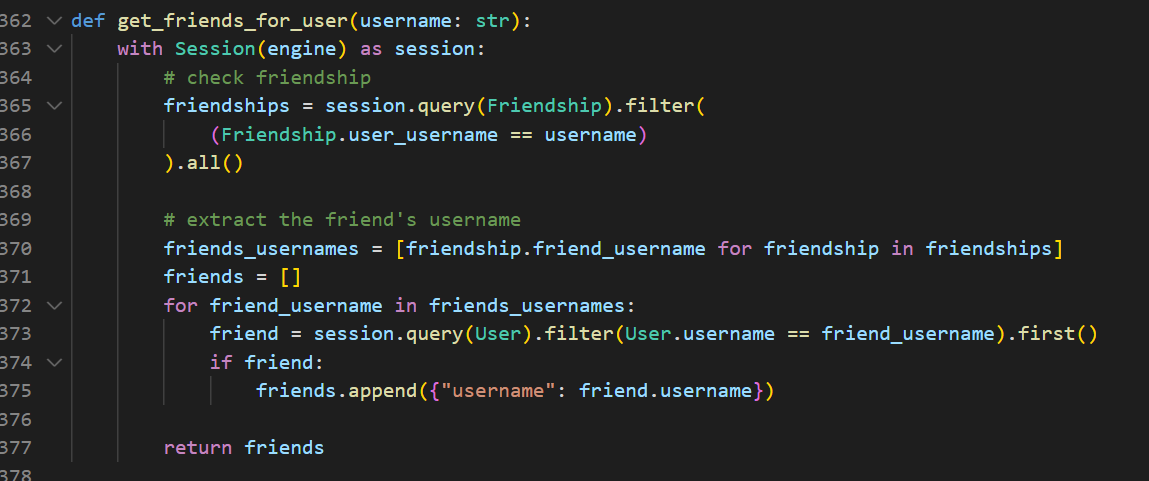
\includegraphics[width=0.8\textwidth]{zzrgraphs/db_getfriendforuser.png}
                \caption{db.py get all the friends of the current user}
                \label{getfriends}
            \end{figure}

        \begin{figure}[H]
                \centering
                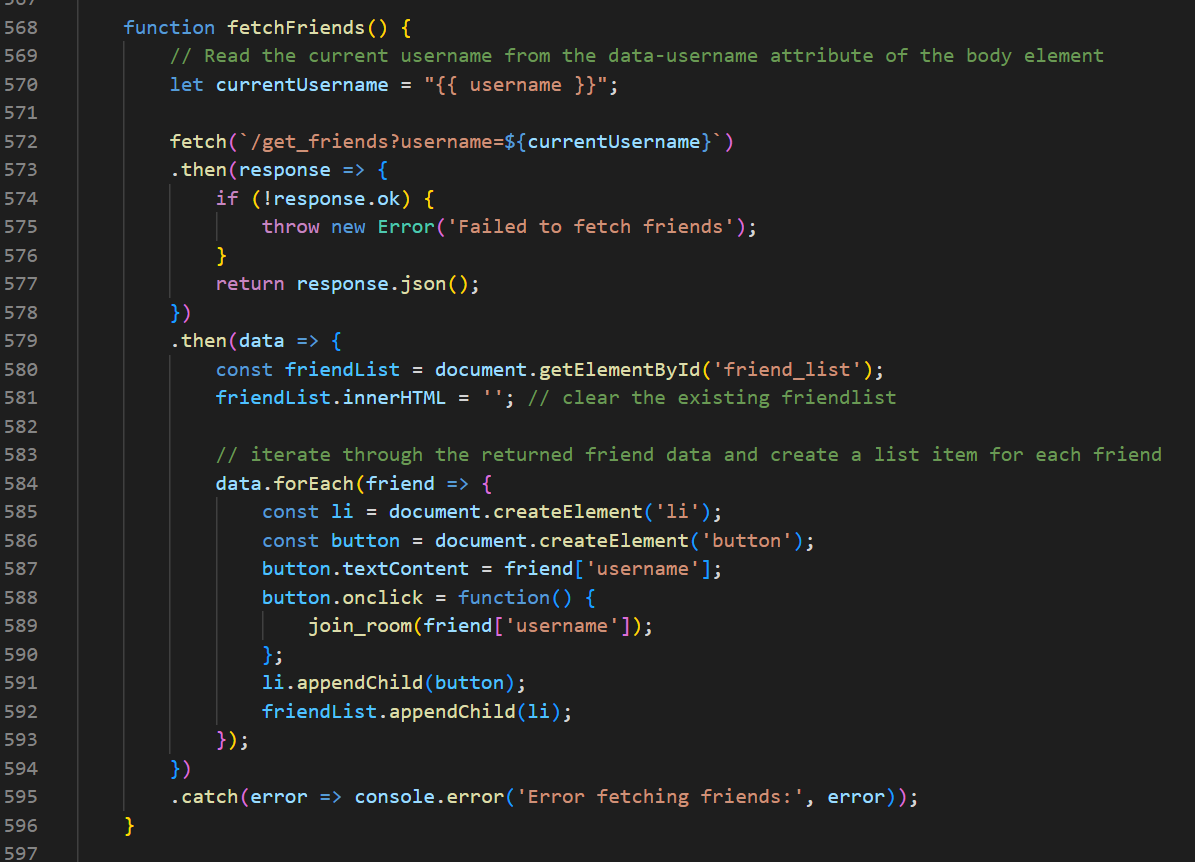
\includegraphics[width=0.8\textwidth]{zzrgraphs/home_fetchFriends.png}
                \caption{home.jinja fetch friends function}
                \label{fetchfriends}
            \end{figure}

        \subsubsection*{3} The user can send a friend request to the other user by entering the username(shown in Figure \ref{enterusername}). We designed a class called FriendRequest to implement this feature (shown in Figure \ref{friendrequestClass}). Once entering the username, the server will check whether the username exists. If the username is valid, then it will check whether they are already been friends\ref{sendfriendrequest}. If so, the friend request will not be sent.

        \begin{figure}[H]
                \centering
                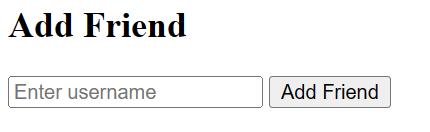
\includegraphics[width=0.4\textwidth]{zzrgraphs/enter_username.png}
                \caption{home page: add friend feature}
                \label{enterusername}
            \end{figure}

        \begin{figure}[H]
                \centering
                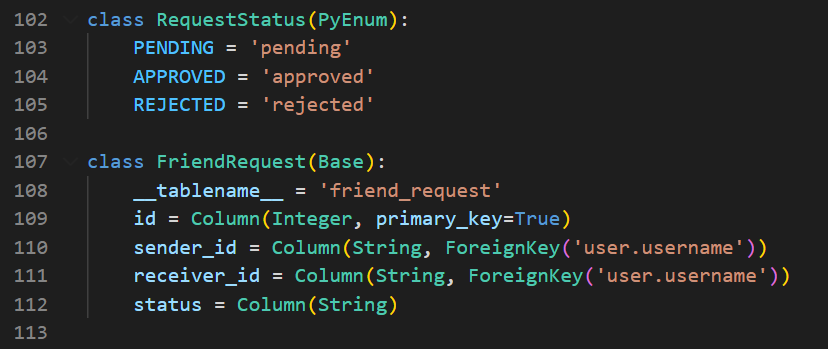
\includegraphics[width=0.8\textwidth]{zzrgraphs/models_friendrequest.png}
                \caption{models.py define a class called friendrequest}
                \label{friendrequestClass}
            \end{figure}

        \begin{figure}[H]
                \centering
                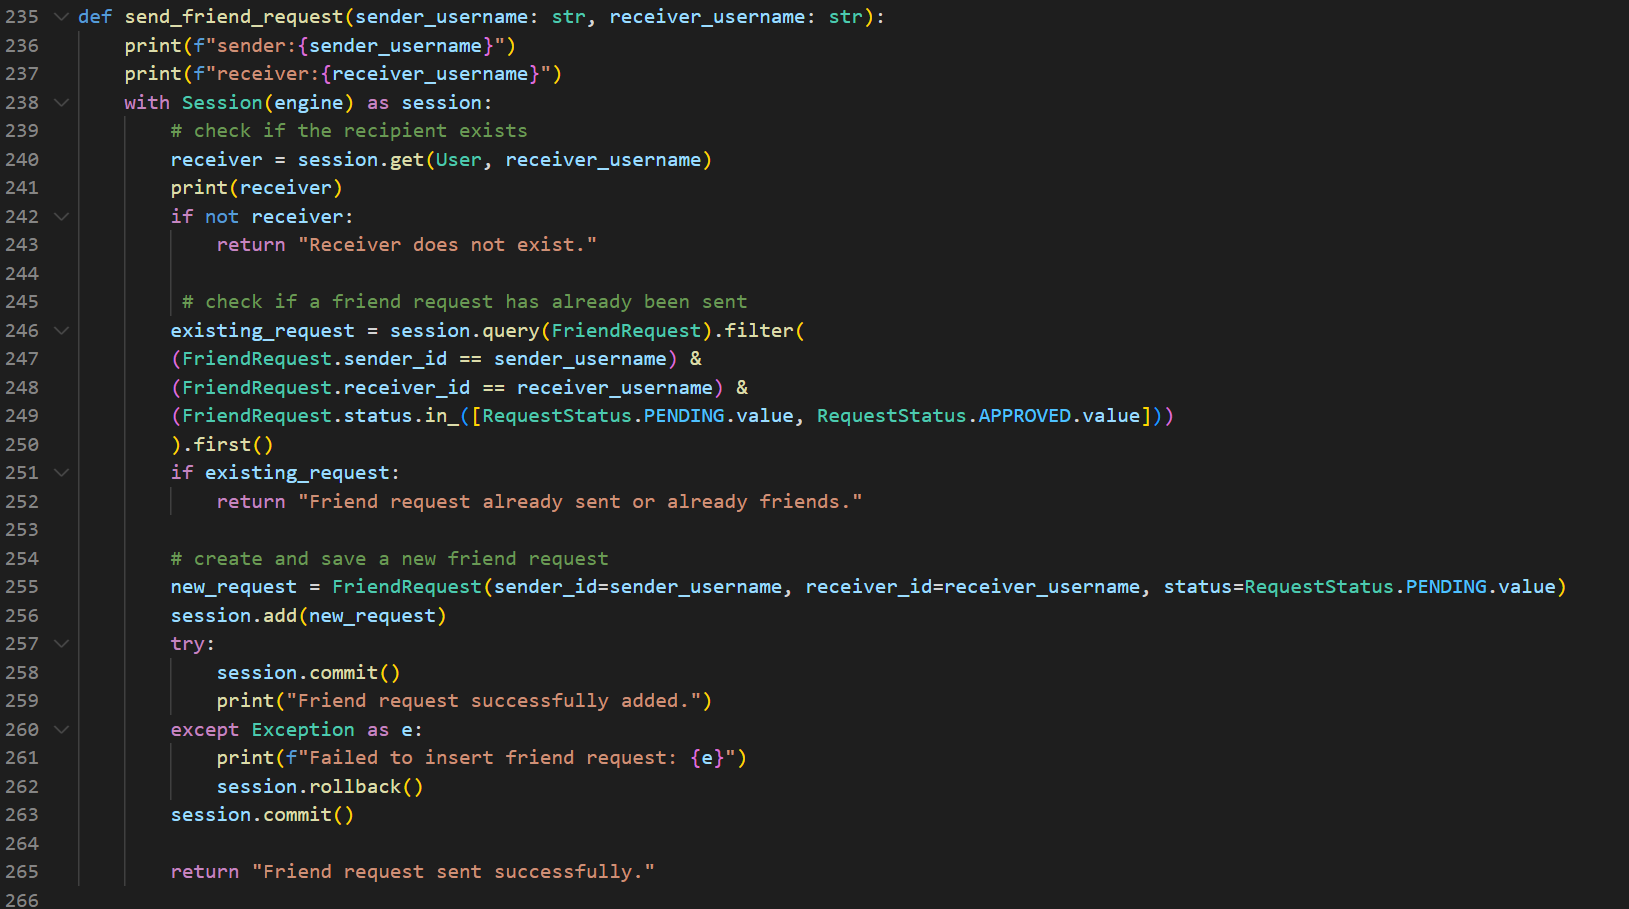
\includegraphics[width=0.8\textwidth]{zzrgraphs/db_send_friend_request.png}
                \caption{db.py send friend request to the other user}
                \label{sendfriendrequest}
            \end{figure}
	
	   \subsubsection*{4} Once the user trying to send a friend request, if the users are already friends, the request will not be send and will not be displayed. Otherwise, the request will be displayed dynamically to both sender and receiver. The sender will see a message which shows "To: receiver", while the receiver will see "From: sender", with two buttons "Accept" and "Reject"(shown in Figure \ref{twobuttons}) . Once the receiver accept the friendship request, the status will be updated \ref{updatestatus} , and the receiver will become a friend of the sender and will be shown in the friend list immediately. Otherwise if the receiver reject the request, the status will also be updated immediately and this request will disappear automatically.  In order to achieve the dynamic part, we applyed socket to listen to the friendrequest(shown in Figure  \ref{fetchrequests} Figure \ref{requestsocketio}) , so it will update the friend requests automatically without manual refresh.

        \begin{figure}[H]
                \centering
                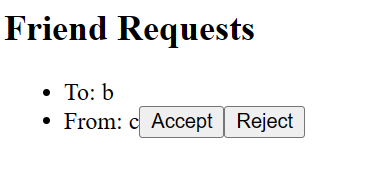
\includegraphics[width=0.4\textwidth]{zzrgraphs/display_friendrequests.png}
                \caption{home page: display friend requests}
                \label{twobuttons}
            \end{figure}

        \begin{figure}[H]
                \centering
                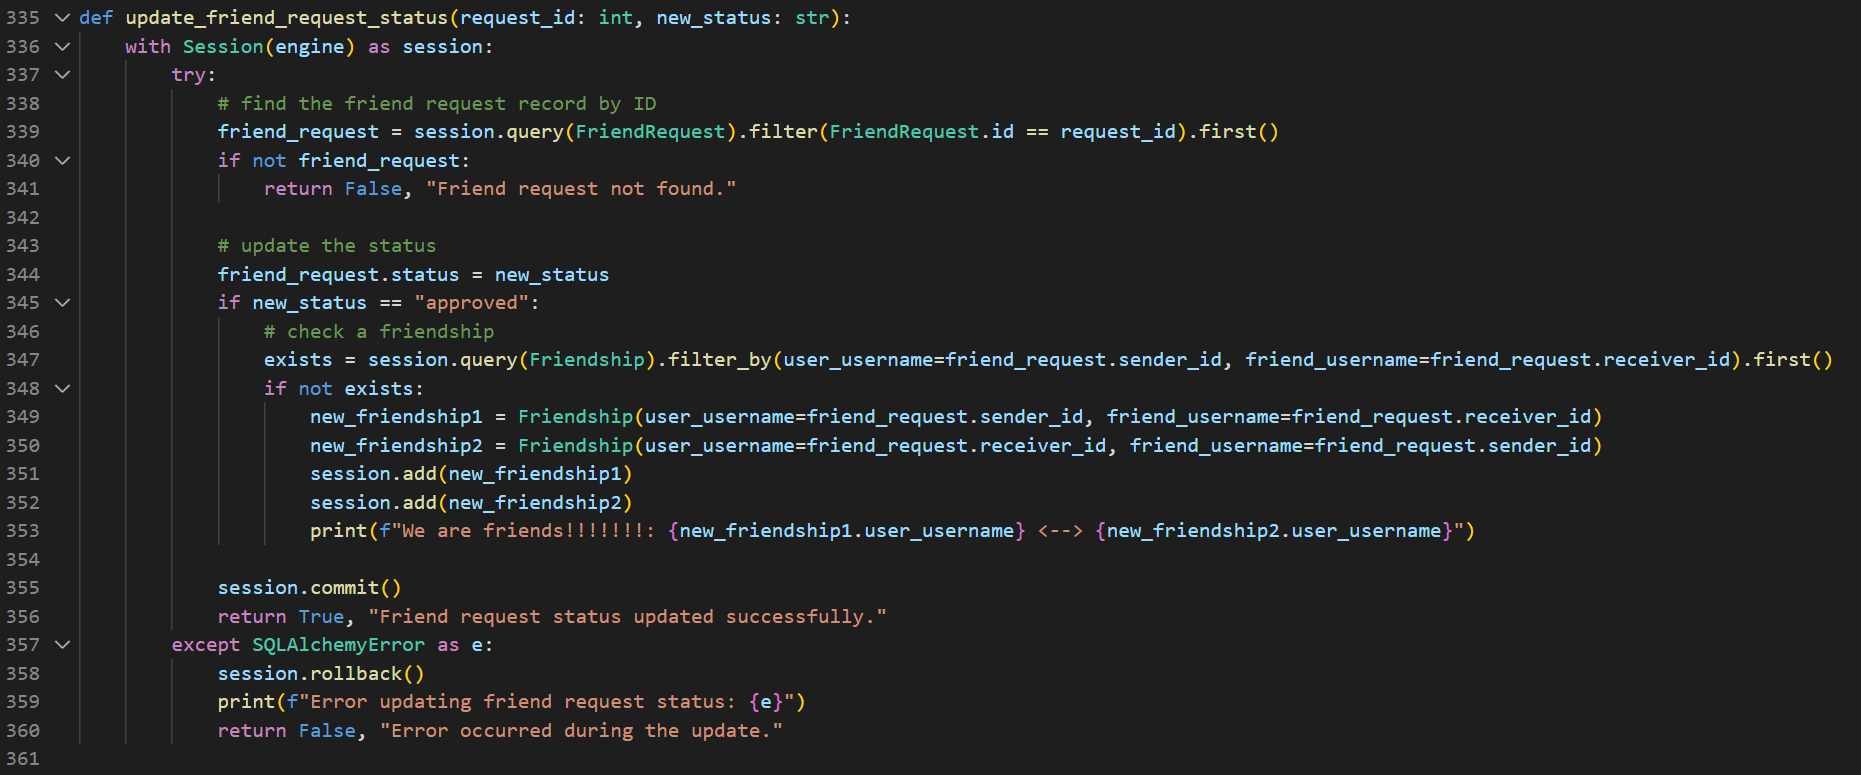
\includegraphics[width=0.8\textwidth]{zzrgraphs/db_update_request_status.png}
                \caption{db.py: update request status after user's operation}
                \label{updatestatus}
            \end{figure}

        \begin{figure}[H]
                \centering
                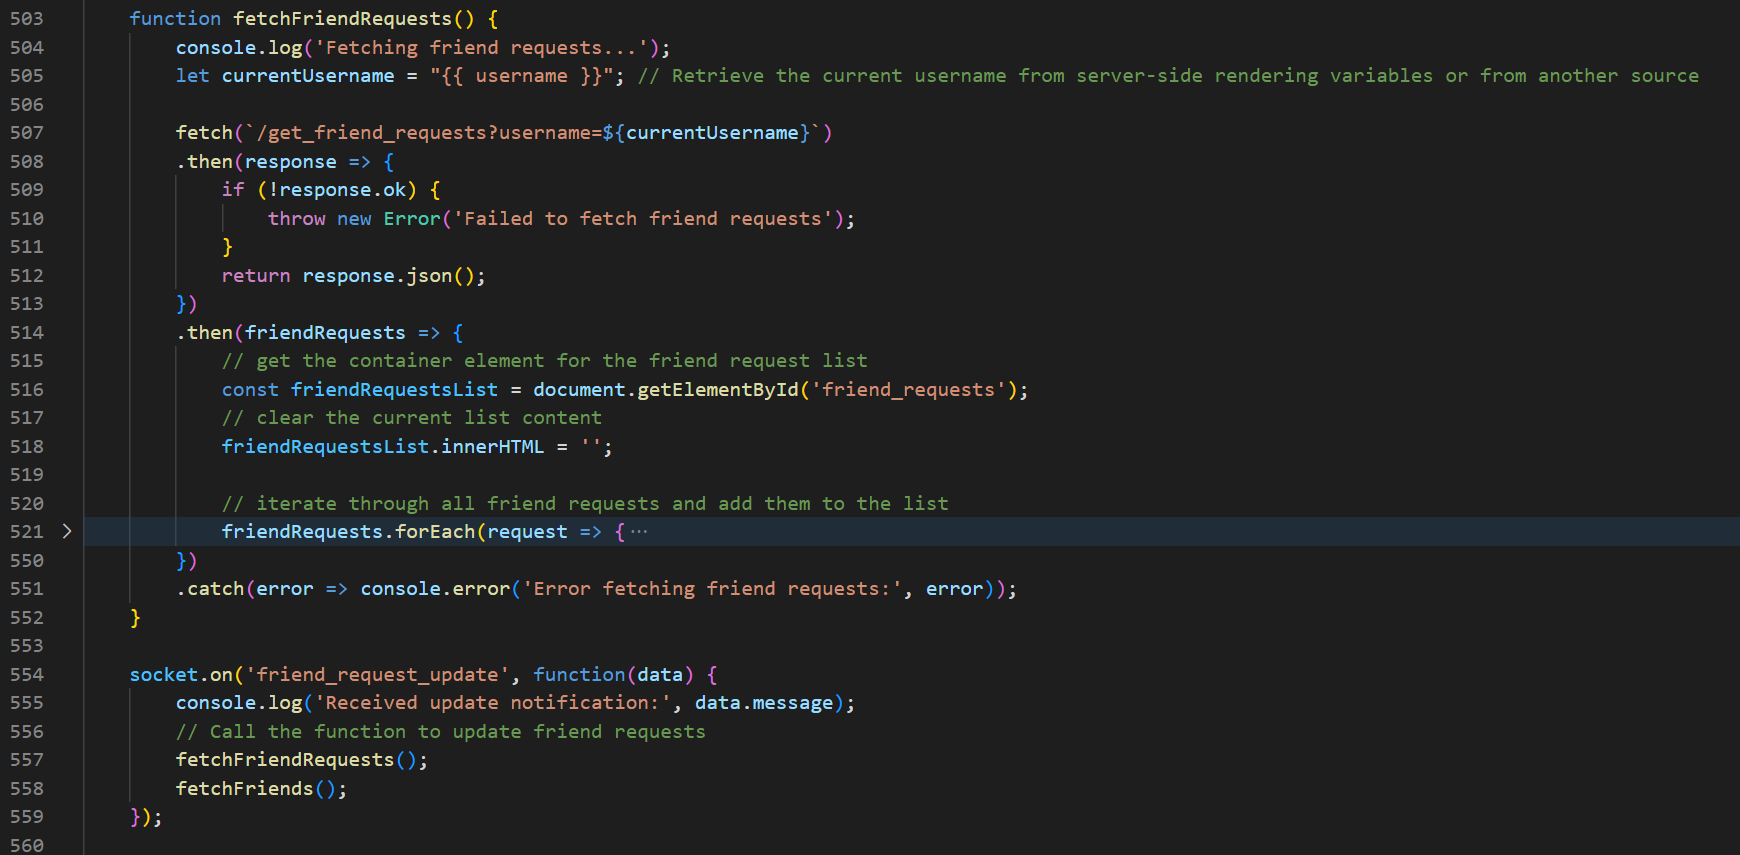
\includegraphics[width=0.8\textwidth]{zzrgraphs/home_fetchfriendrequests.png}
                \caption{home.jinja: fetch friendrequests and socket}
                \label{fetchrequests}
            \end{figure}
    
        \begin{figure}[H]
                \centering
                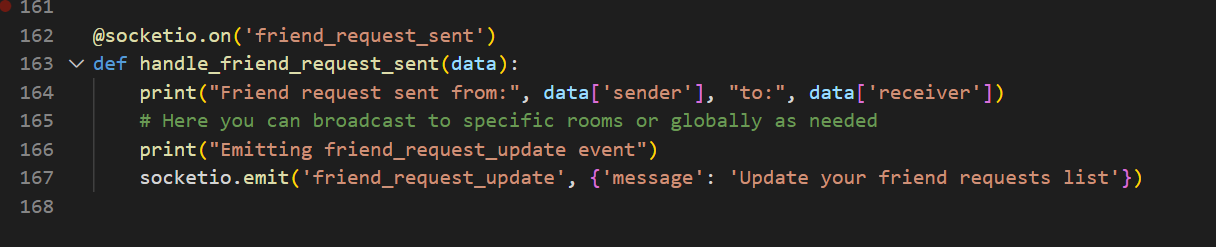
\includegraphics[width=0.8\textwidth]{zzrgraphs/socket_friend_request_sent.png}
                \caption{socket routes.py: listen to the frontend}
                \label{requestsocketio}
            \end{figure}

        \subsubsection*{5} 

        All the friends of the user is displayed as buttons in the friend list (shown in Figure \ref{friendlist}).  Once clicking on the button, it will call the join room function which allows the user to join in their friend's chat room.  To ensure that both user and friend are currently on so they can communicate securely, we add a get users in room medthod for the room class, which checks whether both of them are in the room.(shown in Figure \ref{getusersinroom}). Then we use this method when trying to send messages (shown in Figure \ref{send}).


        \begin{figure}[H]
                \centering
                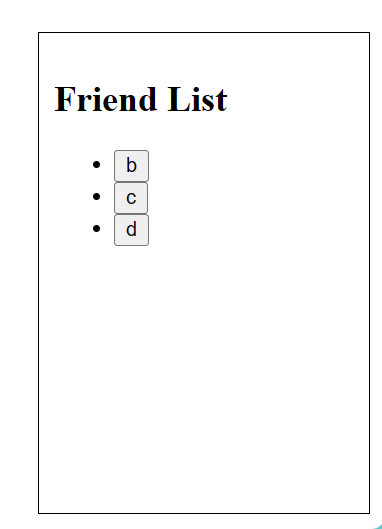
\includegraphics[width=0.2\textwidth]{zzrgraphs/friend_list.png}
                \caption{home page: friends are displayed as buttons}
                \label{friendlist}
            \end{figure}

        \begin{figure}[H]
            \centering
            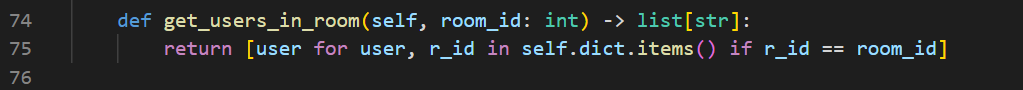
\includegraphics[width=0.8\textwidth]{zzrgraphs/models_get_users_in_room.png}
            \caption{models.py: check how many users are in the room}
            \label{getusersinroom}
        \end{figure} 

        \begin{figure}[H]
            \centering
            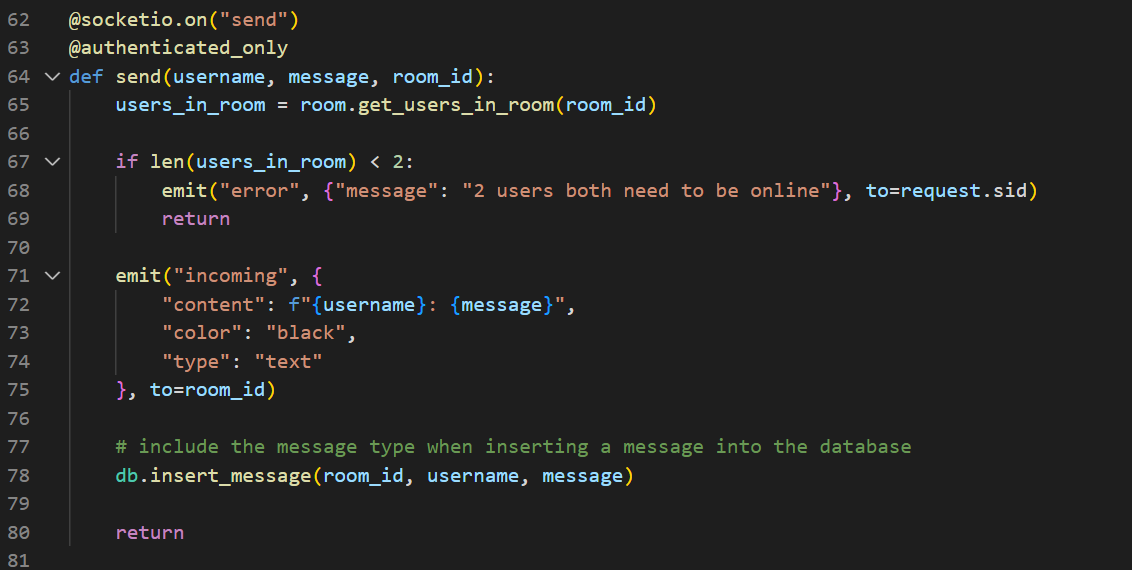
\includegraphics[width=0.8\textwidth]{zzrgraphs/socket_send.png}
            \caption{socket routes.py: check whether both users are online before sending message}
            \label{send}
        \end{figure}  

        \textbf{The process of ensuring secure communication between users:}
        \begin{enumerate}
            \item When a user successfully logs in or signs up, they generate a pair of cryptographic keys: a public key and a private key as shown in Figure \ref{show_keys}.

            As shown in Figure \ref{generate_key_pairs}, the process begins with hashing the password using the SHA-256 hash function to create a fixed-length seed. This enhances security by mitigating risks associated with using raw passwords and provides necessary entropy. The SHA-256 hash output, initially an ArrayBuffer, is then converted into a Uint8Array, and finally into a hexadecimal string to format the seed for key generation. Using this processed seed, the ec.genKeyPair function from the elliptic library is utilized to generate the  key pair.
            
            Subsequently, the frontend stores both the public key and the private key as shown in \ref{store_key_pairs}. The public key is uploaded to the server using an axios request and stored in a database called public\_keys, as shown in Figures \ref{Upload and Store public key} and \ref{db public_key}. Meanwhile, the private key is retained in the user's local storage, as shown in Figure \ref{local_storage}. These keys are generated based on the user's password, ensuring that they are consistently the same each time they are generated.

            \begin{figure}[H]
                \centering
                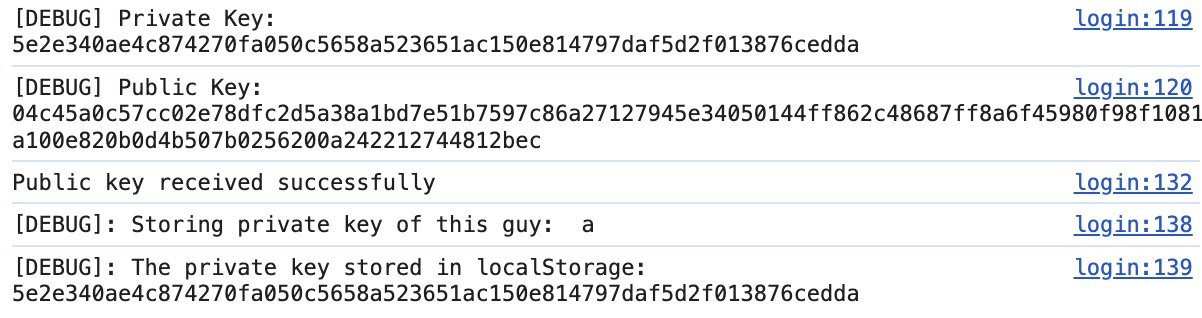
\includegraphics[width=0.8\textwidth]{graphs/show_keys.jpg}
                \caption{Illustration of private and public keys}
                \label{show_keys}
            \end{figure}

            \begin{figure}[H]
                \centering{}
                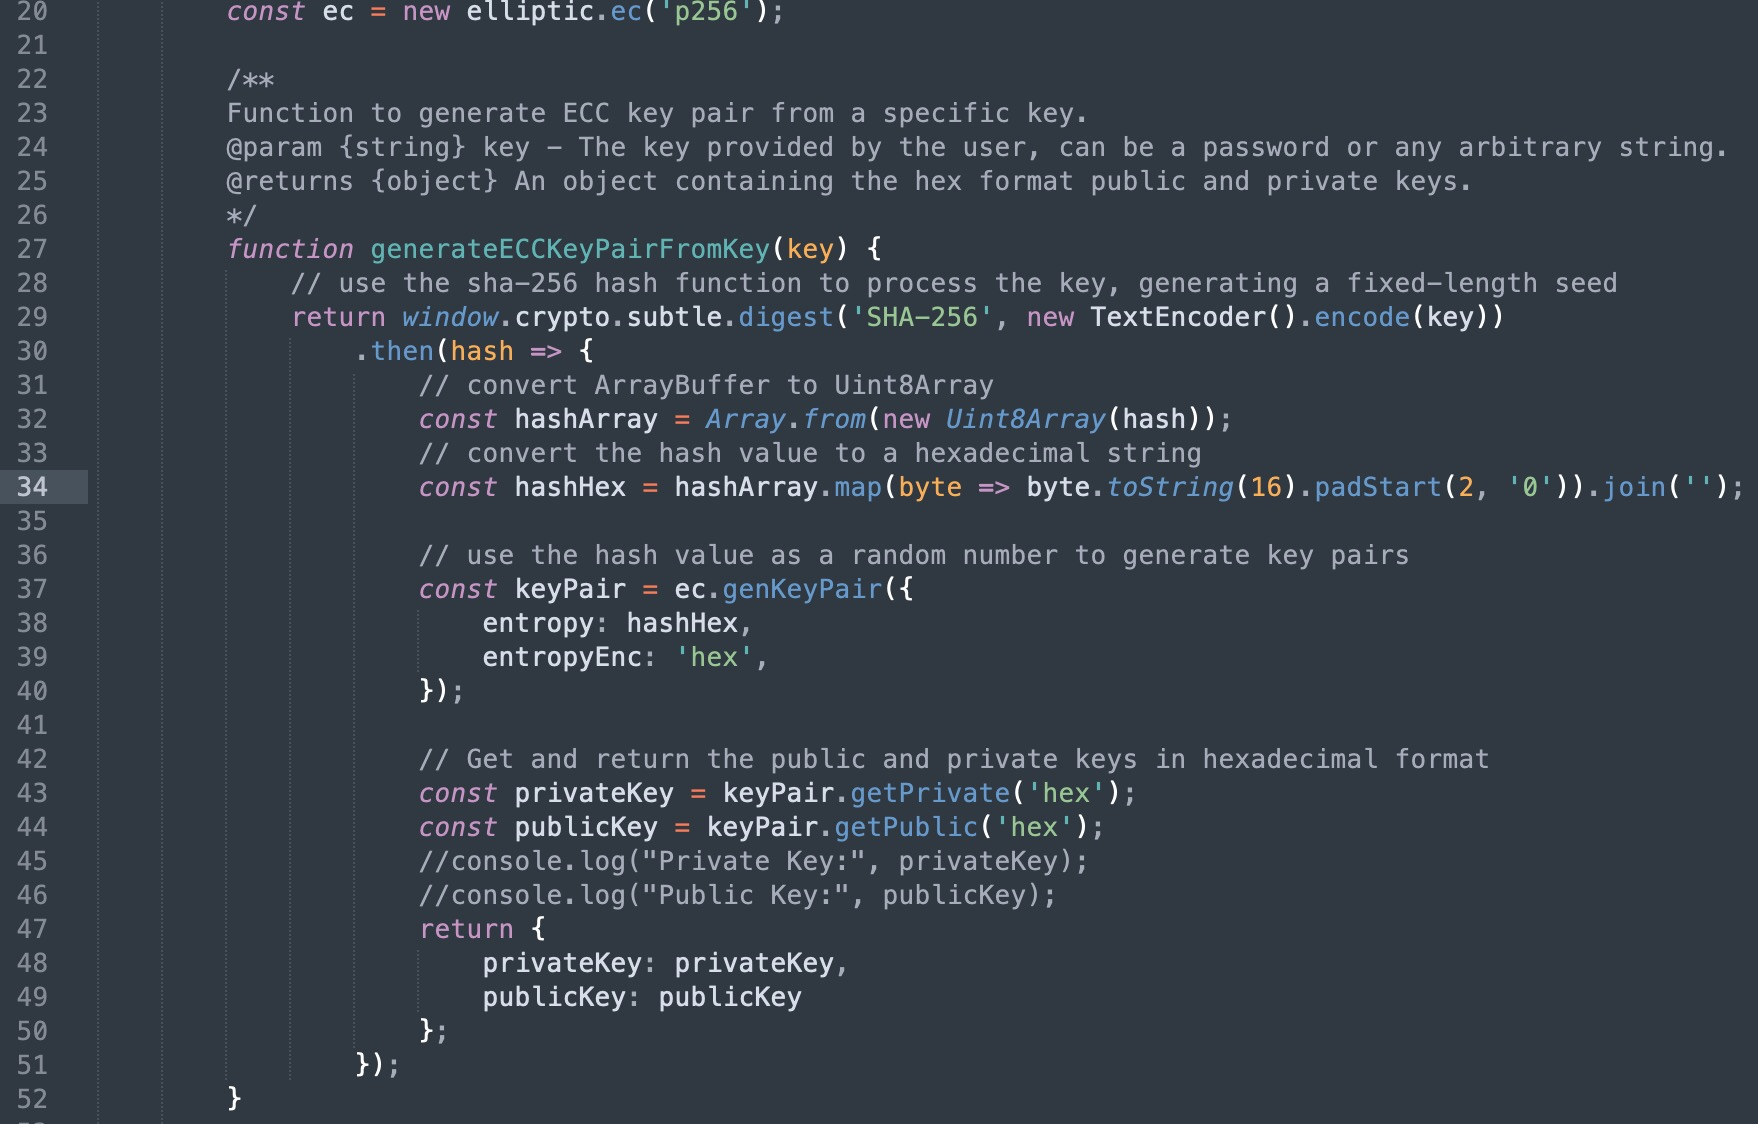
\includegraphics[width=0.8\textwidth]{graphs/generate_key_pairs.jpg}
                \caption{login.jinja and same function in signup.jinja }
                \label{generate_key_pairs}
            \end{figure}

            \begin{figure}[H]
                \centering{}
                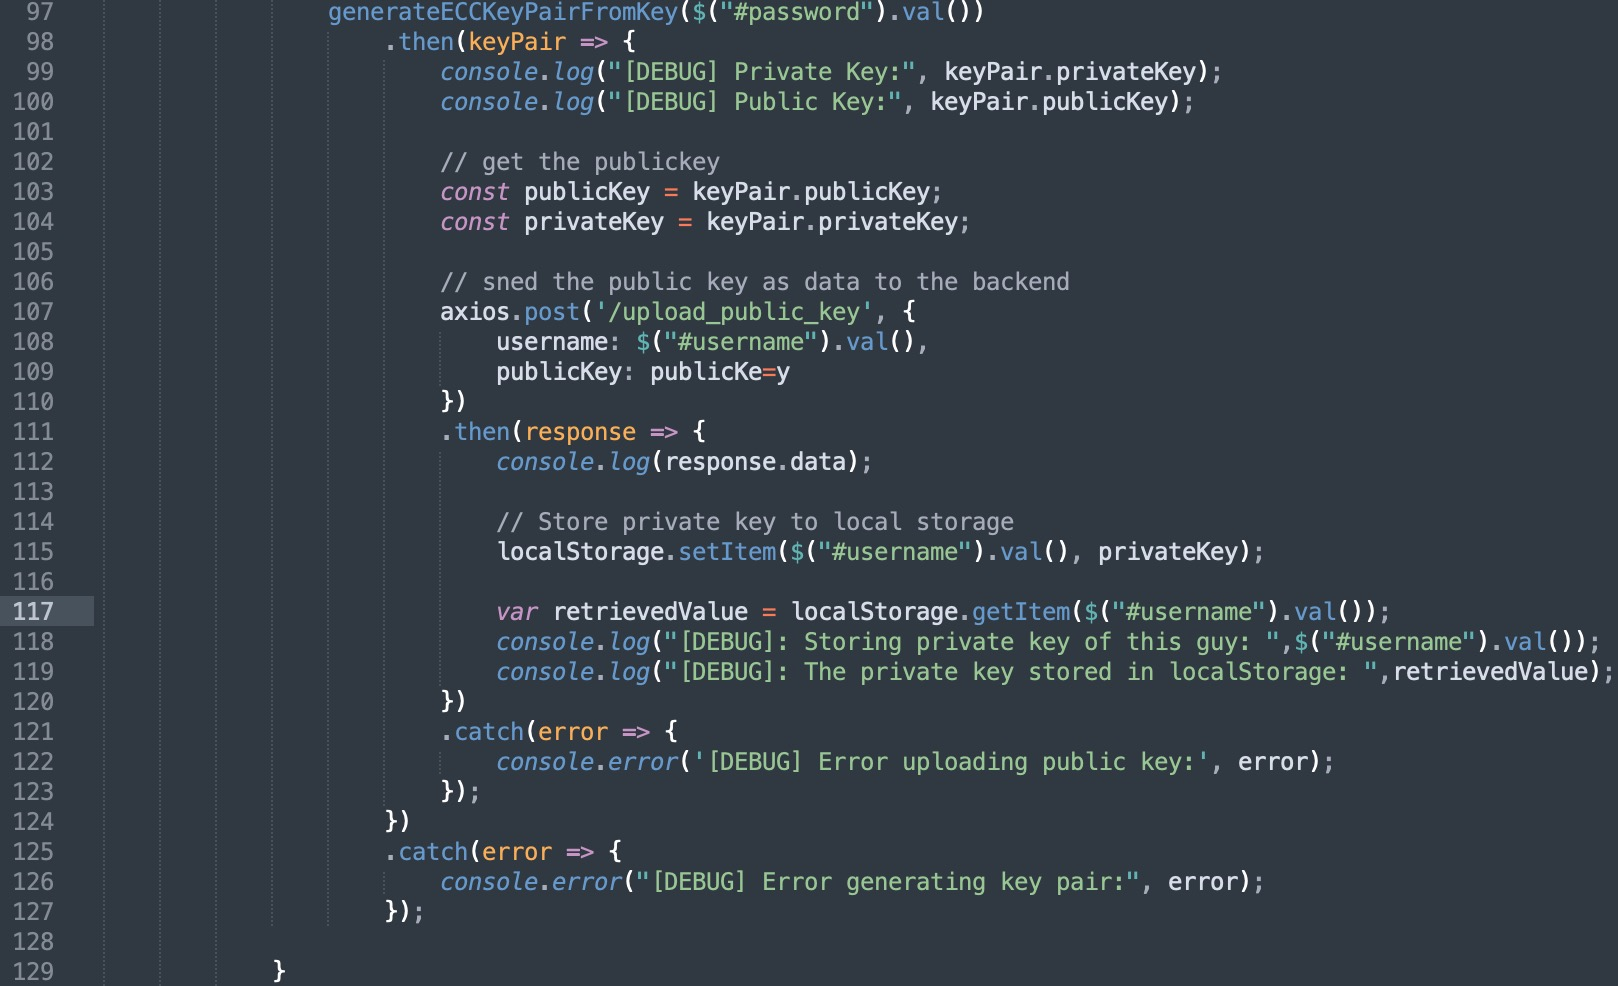
\includegraphics[width=0.7\textwidth]{graphs/store_key_pairs.jpg}
                \caption{login.jinja and same process in signup.jinja }
                \label{store_key_pairs}
            \end{figure}

            \begin{figure}[H]
                \centering
                \begin{subfigure}[b]{0.45\textwidth}
                    \centering
                    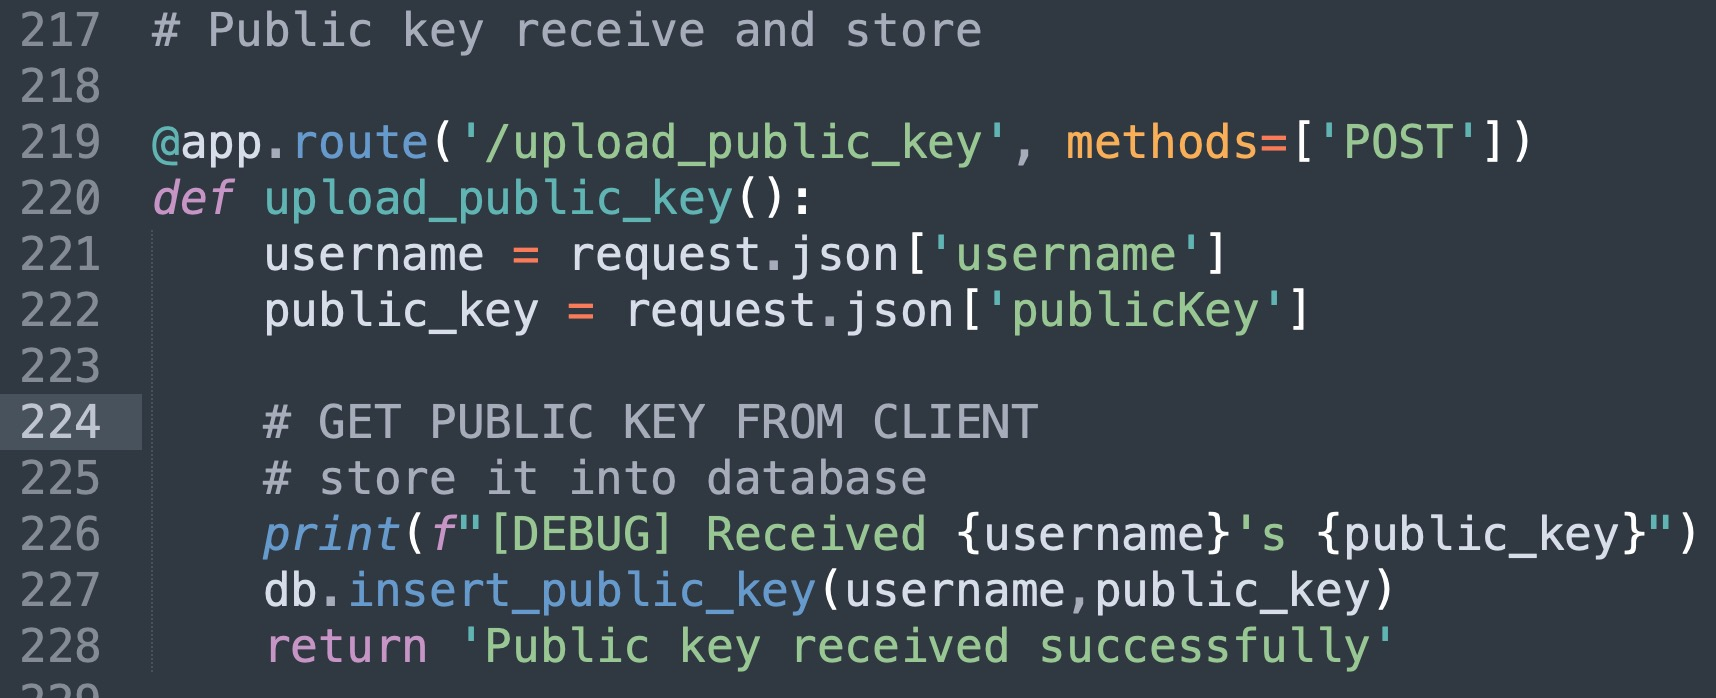
\includegraphics[width=\textwidth]{graphs/upload_public_key.jpg}
                    \caption{upload\_public\_key}
                \end{subfigure}
                \hfill 
                \begin{subfigure}[b]{0.45\textwidth}
                    \centering
                    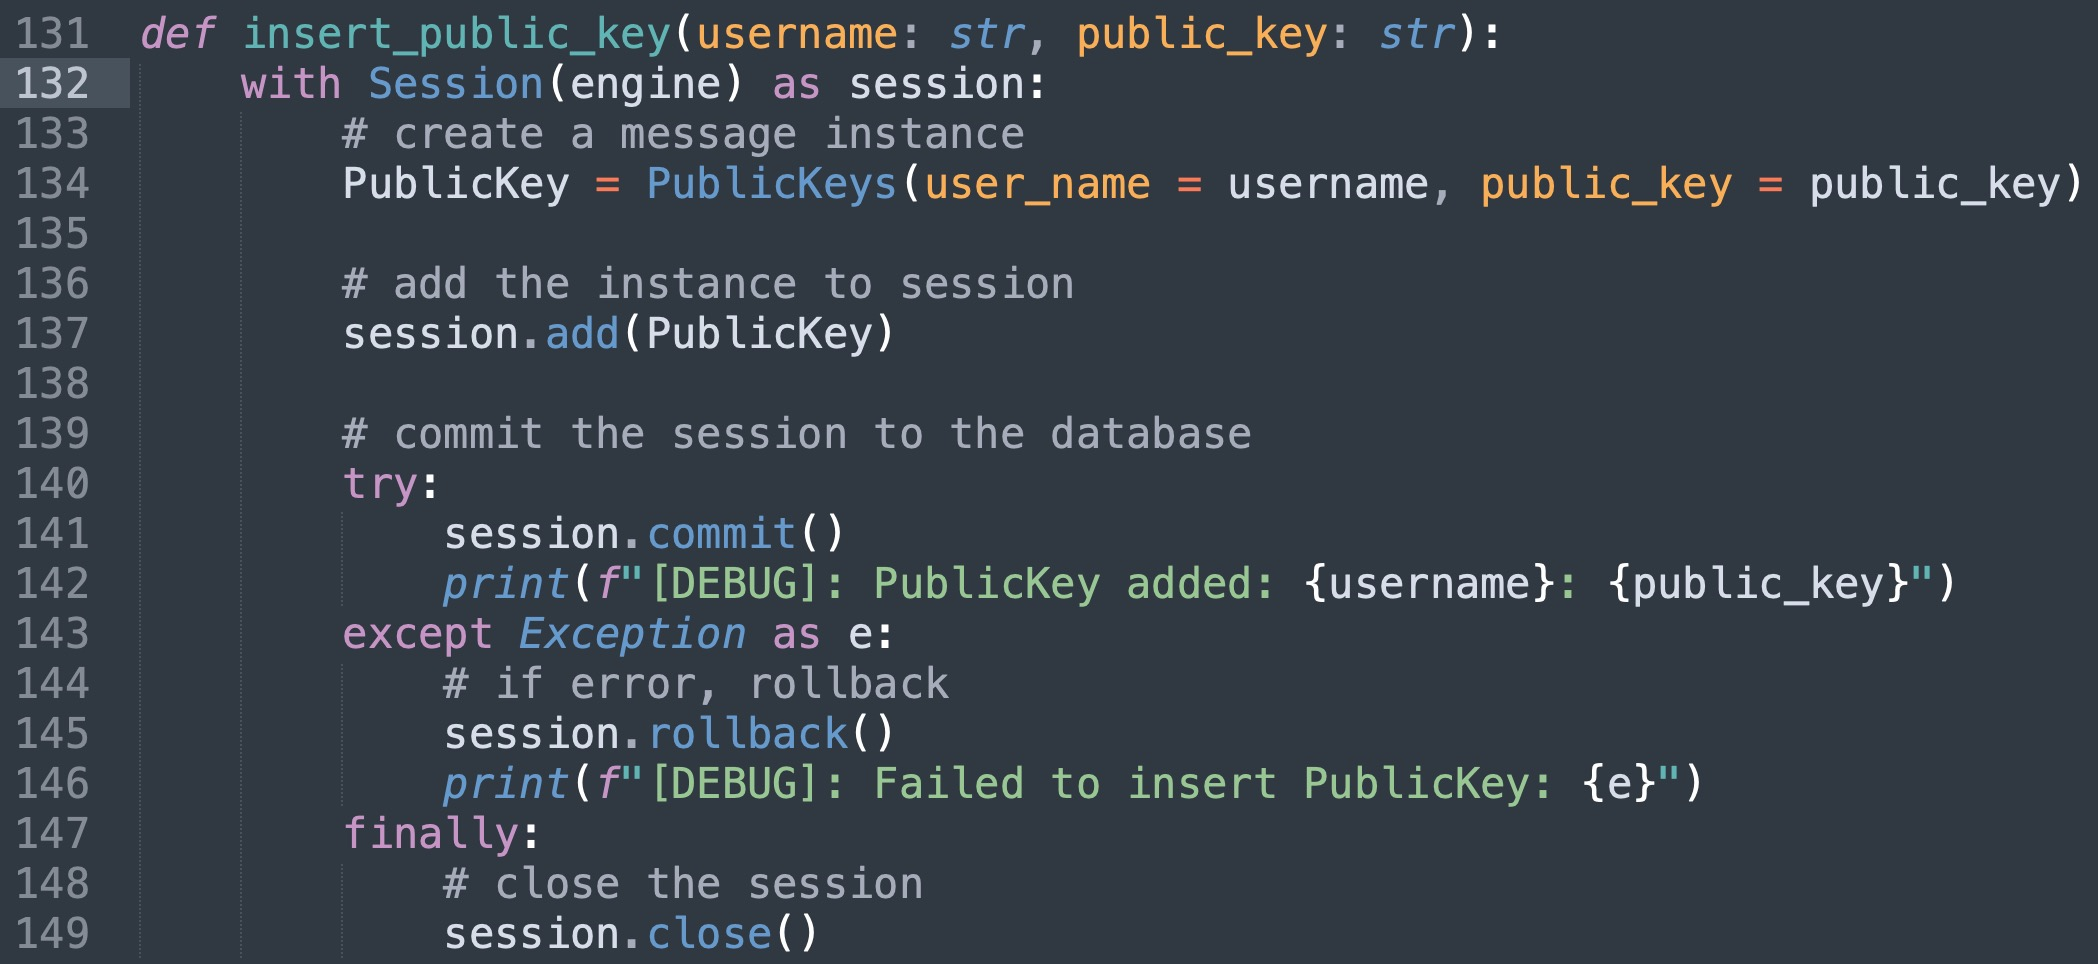
\includegraphics[width=\textwidth]{graphs/insert_public_key.jpg}
                    \caption{insert\_public\_key}
                \end{subfigure}
                \caption{Upload and Store public key}
                \label{Upload and Store public key}
            \end{figure}

            \begin{figure}[H]
                \centering
                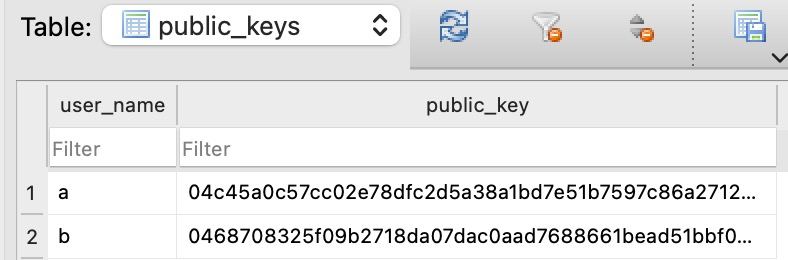
\includegraphics[width=0.8\textwidth]{graphs/db_public_key.jpg}
                \caption{main.db Table: public\_keys}
                \label{db public_key}
            \end{figure}

            \begin{figure}[H]
                \centering
                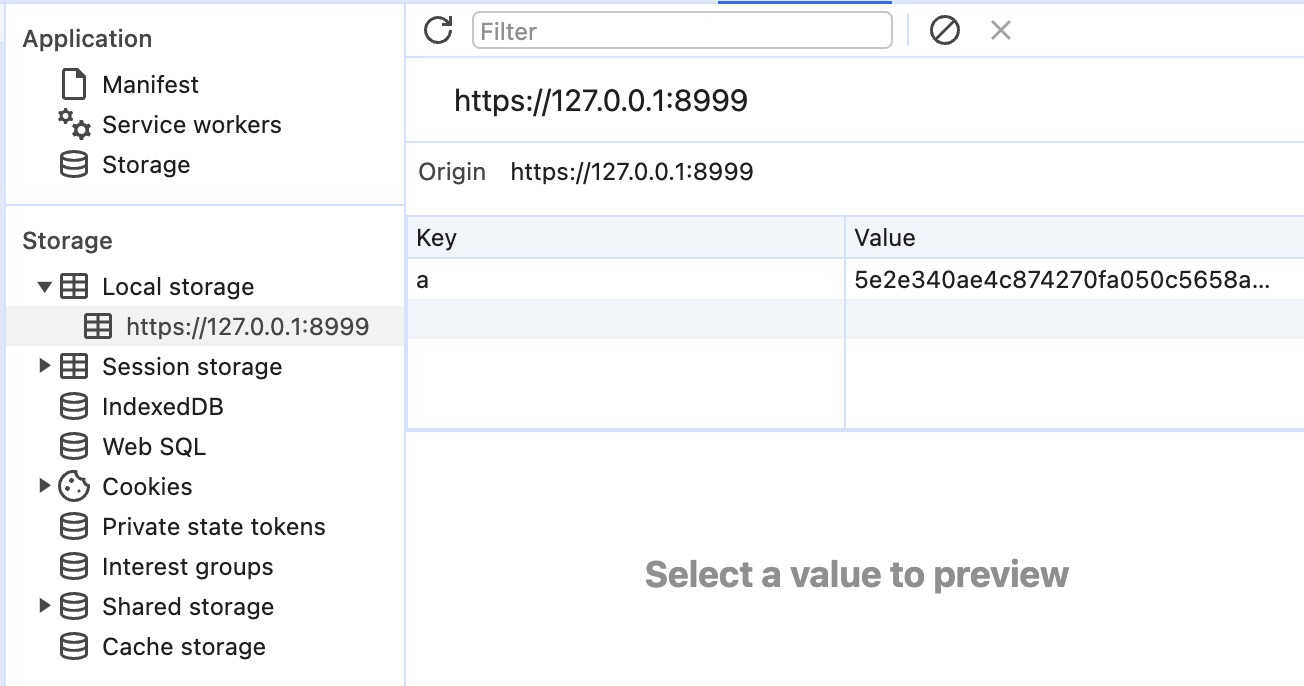
\includegraphics[width=0.8\textwidth]{graphs/local_storage.jpg}
                \caption{main.db Table: public\_keys}
                \label{local_storage}
            \end{figure}

            \item When a user enters a room shown in \ref{front join room}, the function \texttt{getPublicKey(receiver);} shown in \ref{get public key} called to request the public key of the conversing user from the server . The server retrieves the public key from the database and returns it shown in \ref{get and return public key}, storing it in a global variable \texttt{current\_receiver\_public\_key} in \texttt{home.jinja}. 

            When a user sends a message using the \texttt{send} function, they first generate a digital signature, as shown in Figure \ref{sign message}, using their own private key in local storage and the recipient's public key, previously obtained through \texttt{getPublicKey(receiver);} and stored in the global variable in \texttt{home.jinja}. The digital signature is then incorporated into the message itself before it is sent.

            Following this, the function computes a shared key between two users from hexadecimal representations of a private key and a public key, as shown in Figure \ref{compute shared key}. It converts the private key into a key pair object and the public key into a public key object\cite{elliptic_js}. A shared key is then derived using these keys, serving as a secure basis for encrypted communication between the two users. Despite the involvement of individual private keys and the corresponding public key, both parties arrive at the same shared secret key,also know as Diffie-Hellman key exchange \cite{gillis_diffie_hellman_2024}. Thus, we successfully obtain a shared key that can be used for encrypting and decrypting messages, having exchanged only the public keys.


            \begin{figure}[H]
                \centering{}
                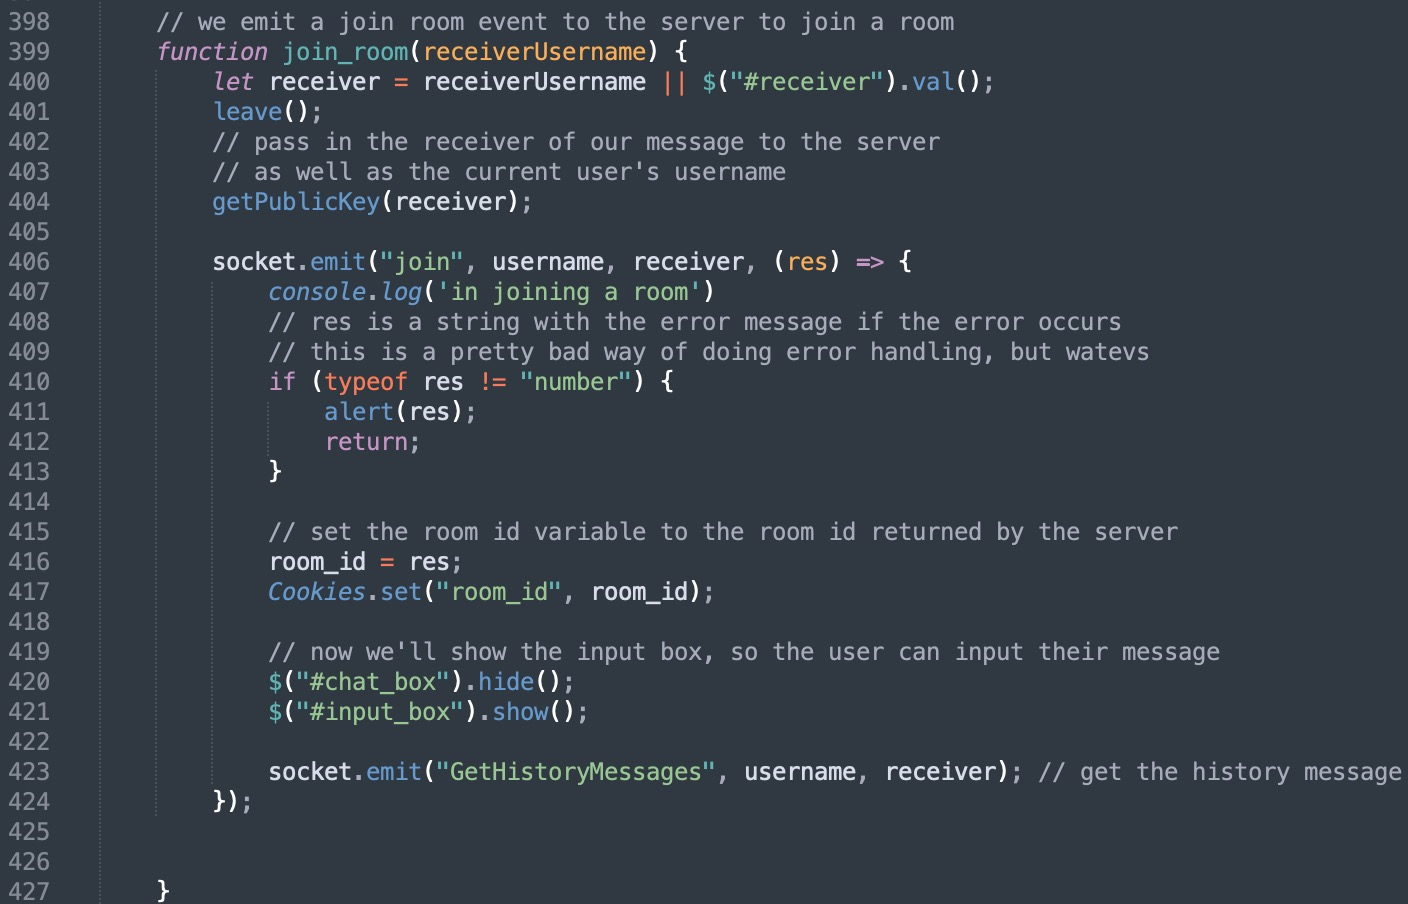
\includegraphics[width=0.8\textwidth]{graphs/front_join_room.jpg}
                \caption{home.jinja join\_room}
                \label{front join room}
            \end{figure}

            \begin{figure}[H]
                \centering
                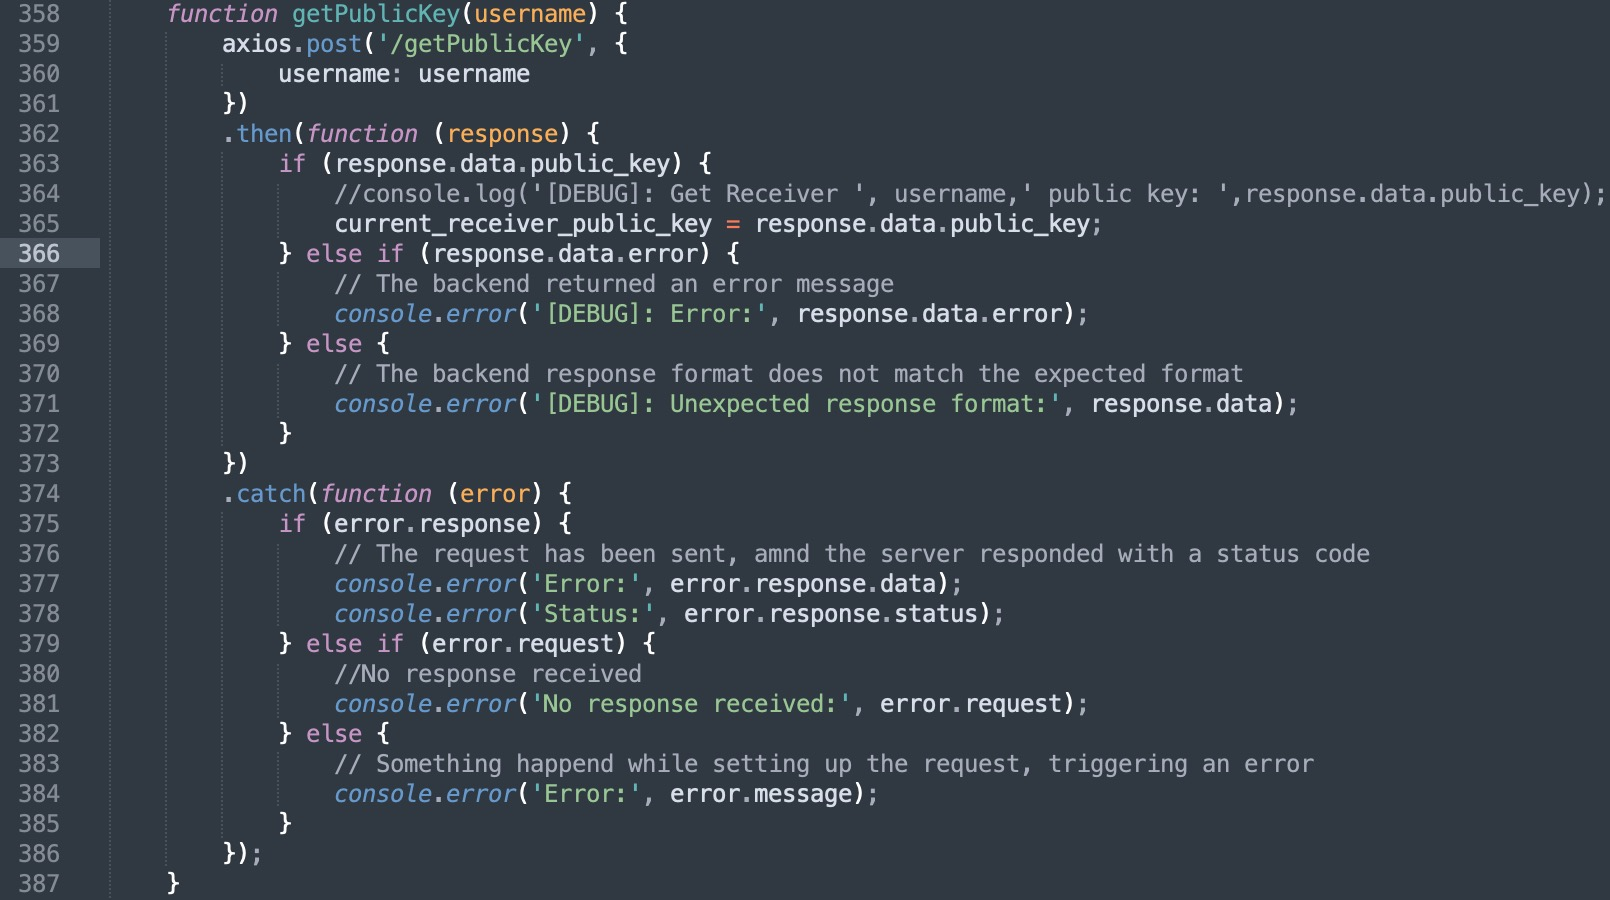
\includegraphics[width=0.8\textwidth]{graphs/front_get_public_key}
                \caption{home.jinja get\_public\_key}
                \label{get public key}
            \end{figure}


            \begin{figure}[H]
                \centering
                \begin{subfigure}[b]{0.47\textwidth}
                    \centering
                    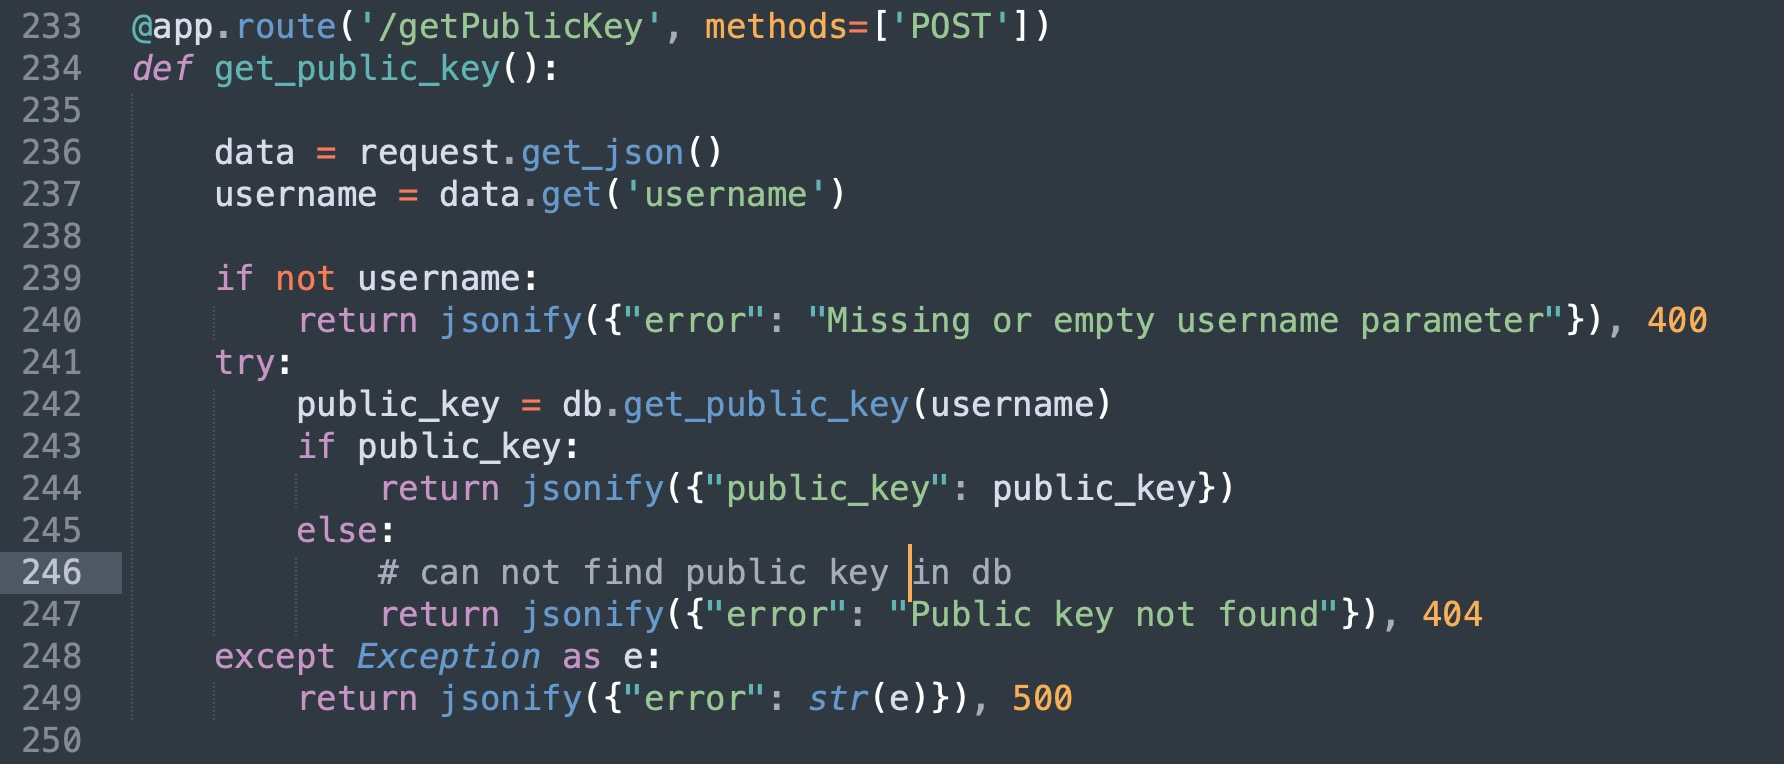
\includegraphics[width=\textwidth]{graphs/back_get_public_key.jpg}
                    \caption{app.py get\_public\_key \textit{line 230 - 246}}
                \end{subfigure}
                \hfill 
                \begin{subfigure}[b]{0.47\textwidth}
                    \centering
                    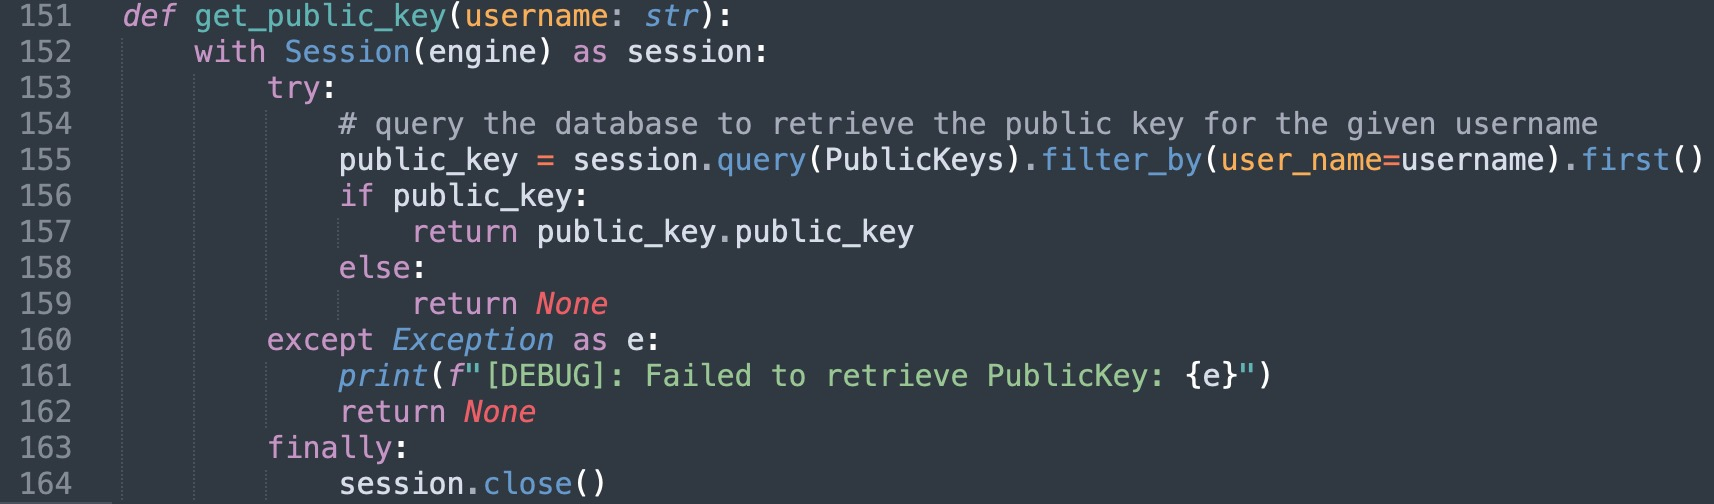
\includegraphics[width=\textwidth]{graphs/db_get_public_key.jpg}
                    \caption{db.py get\_public\_key \textit{line 151 - 164}}
                \end{subfigure}
                \caption{Get and return public key}
                \label{get and return public key}
            \end{figure}

            \begin{figure}[H]
                \centering
                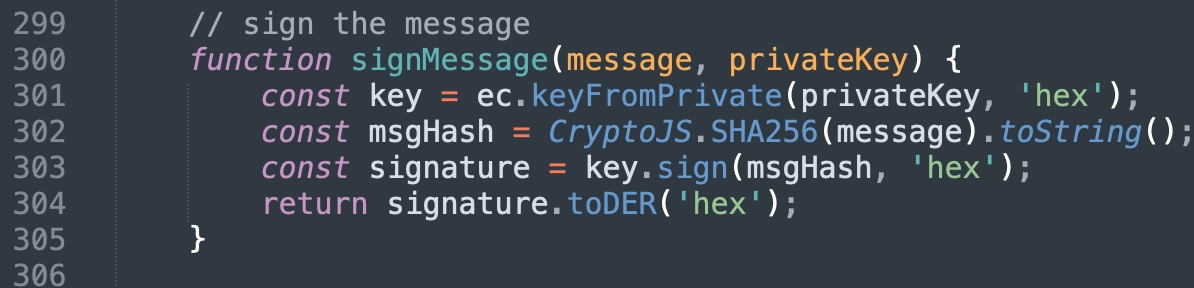
\includegraphics[width=0.8\textwidth]{graphs/sign_message.jpg}
                \caption{home.jinja signMessage \textit{line 299 - 305}}
                \label{sign message}
            \end{figure}

            \begin{figure}[H]
                \centering
                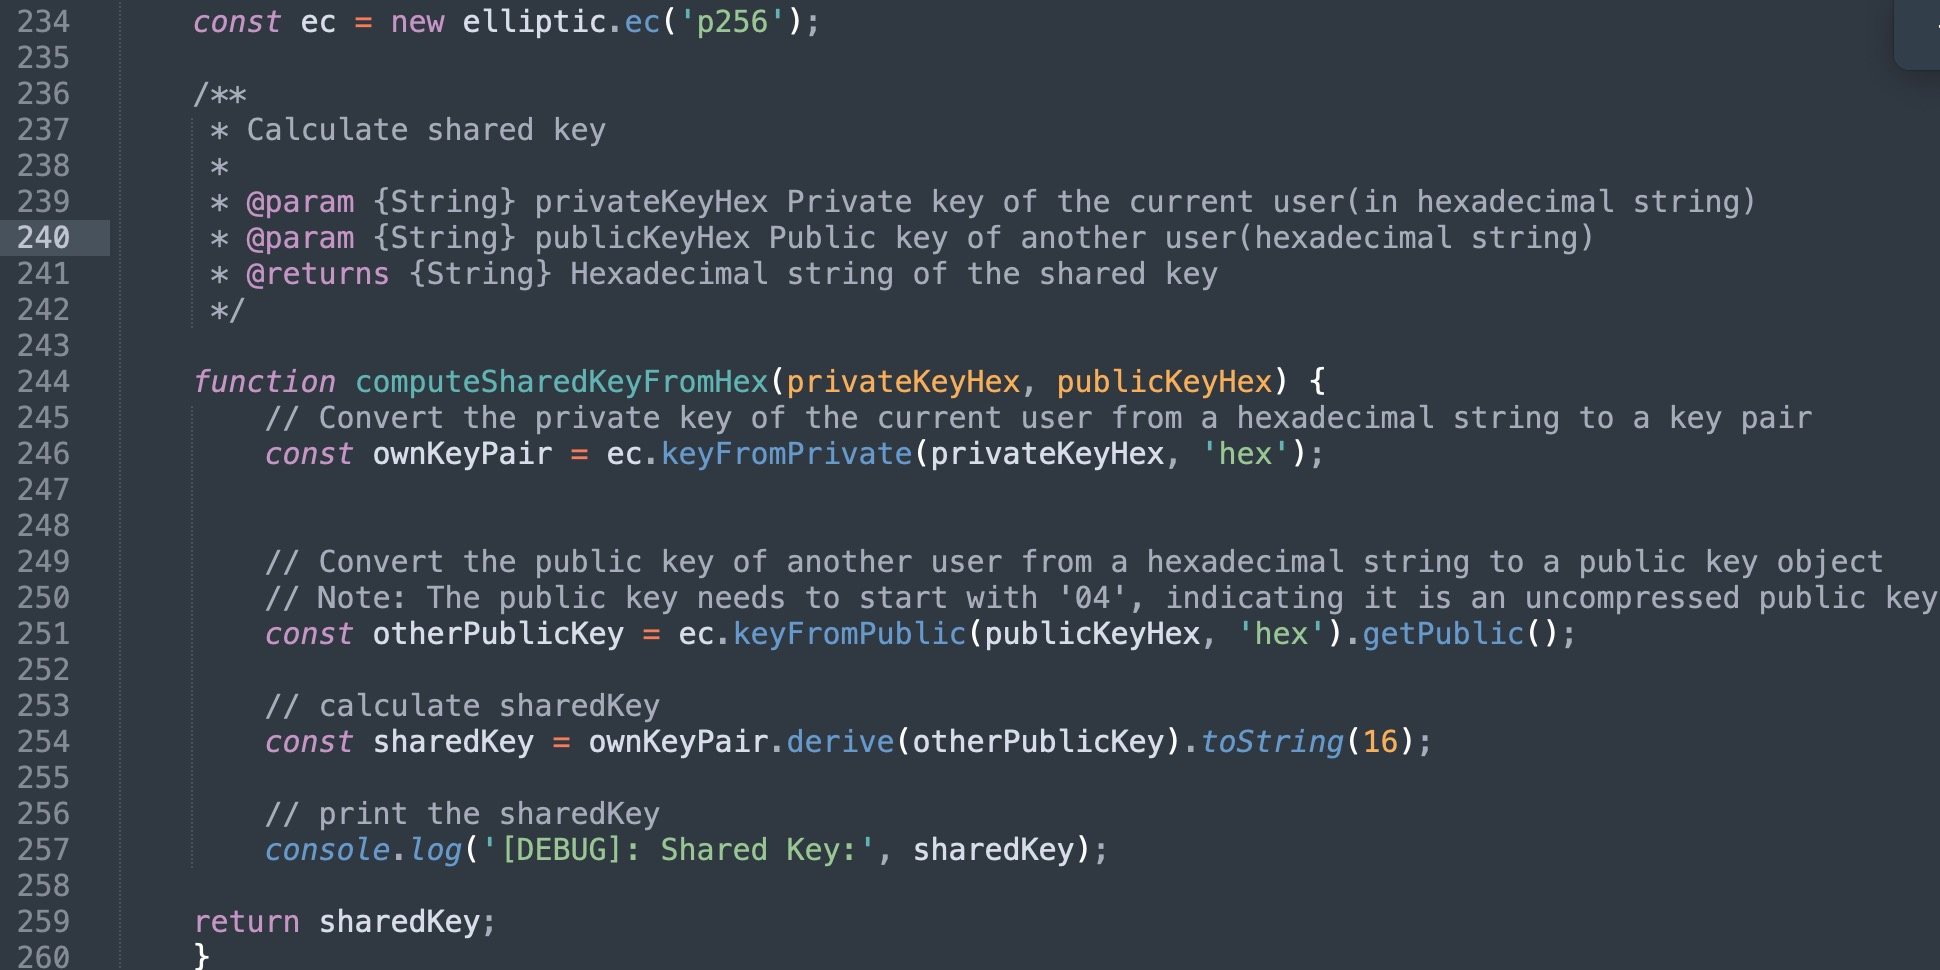
\includegraphics[width=0.8\textwidth]{graphs/compute_shared_key.jpg}
                \caption{home.jinja ComputeSharedKeyFromHex \textit{line 234 - 260}}
                \label{compute shared key}
            \end{figure}


            \item Subsequently, the \texttt{encryptMessage} function is called to encrypt the signed message using the AES algorithm through the CryptoJS library, as shown in \ref{encrypt message}. Initially, the shared key is converted from a hexadecimal string into the format required by the library. Then, the message is encrypted using a specified encryption mode and padding method. Finally, the encrypted, signed message is returned in string form and sent. The server only knows the public key and the encrypted message; thus, even if an attacker gains access to the server, they cannot decipher the message without knowing the user's private key.


            \begin{figure}[H]
                \centering
                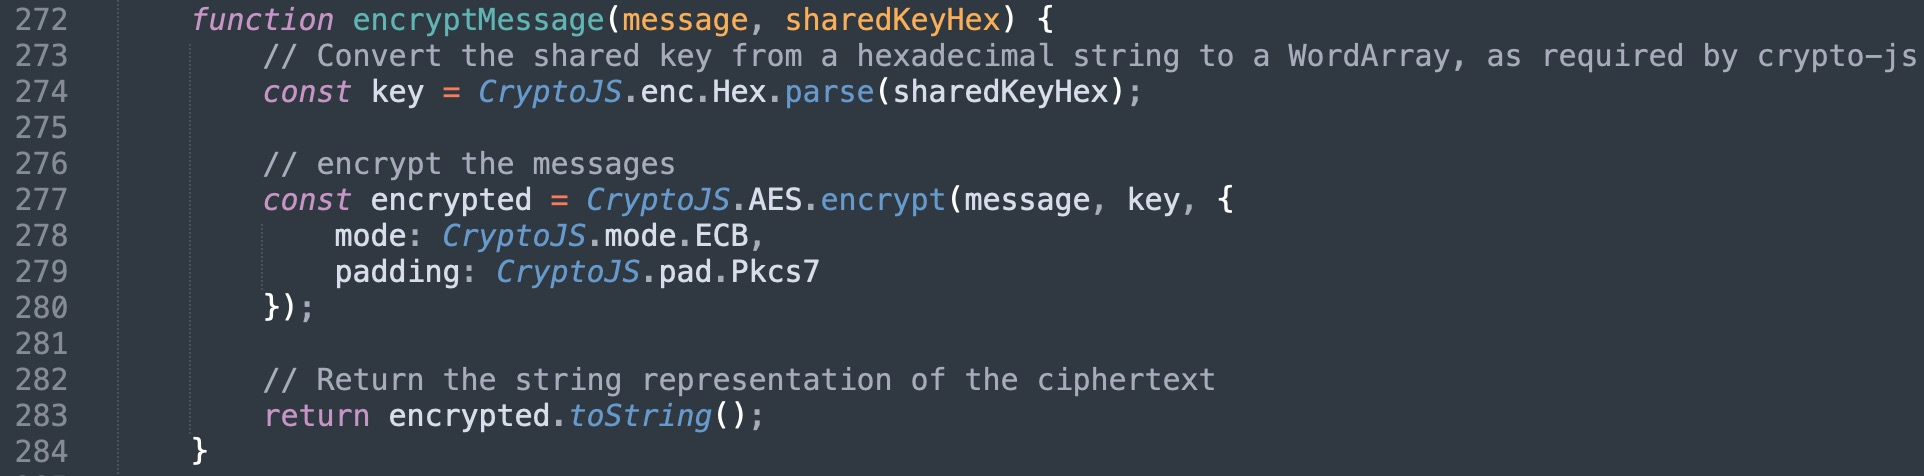
\includegraphics[width=0.8\textwidth]{graphs/encrypt_message.jpg}
                \caption{home.jinja encryptMessage \textit{line 260 - 272}}
                \label{encrypt message}
            \end{figure}

            \item When the recipient receives the encrypted message, the \texttt{incoming} event first calls the \texttt{processMessage} function, as shown in Figure \ref{processMessage}, to decrypt and verify the data. Similar to the previously mentioned process, a shared key is calculated using the sender's public key and the recipient's private key. The message is then decrypted using the \texttt{decryptMessage} function, as shown in Figure \ref{decryptMessage}. Following decryption, the sender's public key is used to verify the signature, as shown in Figure \ref{verify signature}. If all checks are successful, the message is displayed in the message box.The process is shown in Figure \ref{encryption and decryption process}.


            \begin{figure}[H]
                \centering
                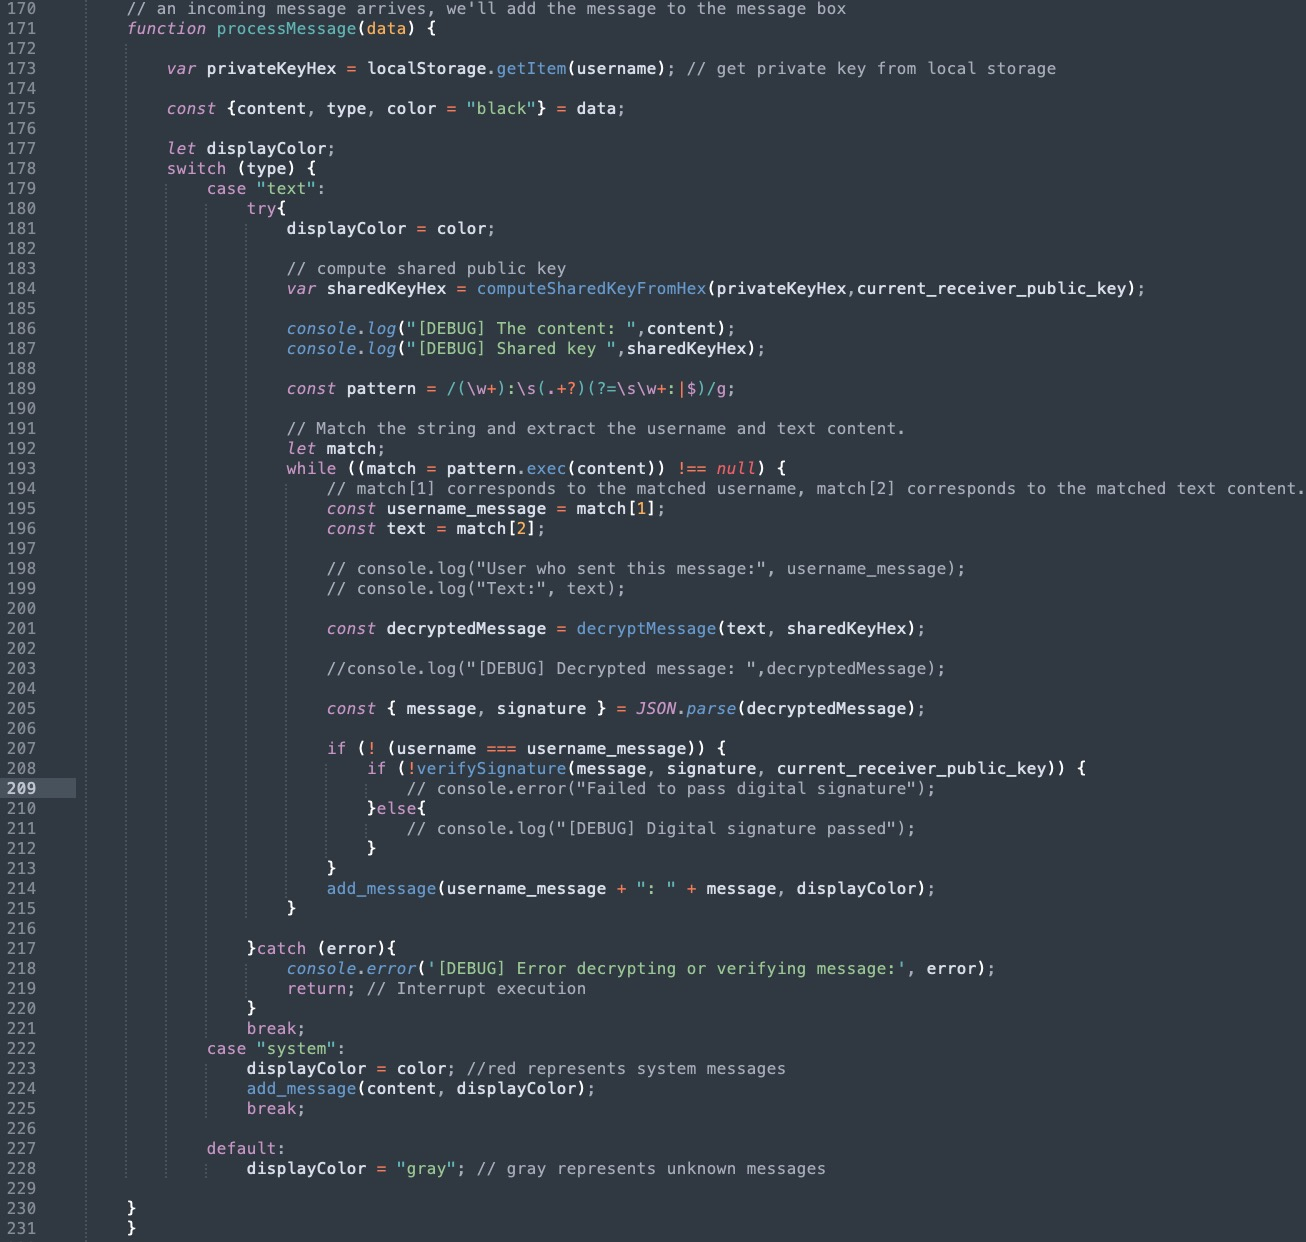
\includegraphics[width=0.8\textwidth]{graphs/processData.jpg}
                \caption{home.jinja processMessage \textit{line 260 - 272}}
                \label{processMessage}
            \end{figure}

            \begin{figure}[H]
                \centering
                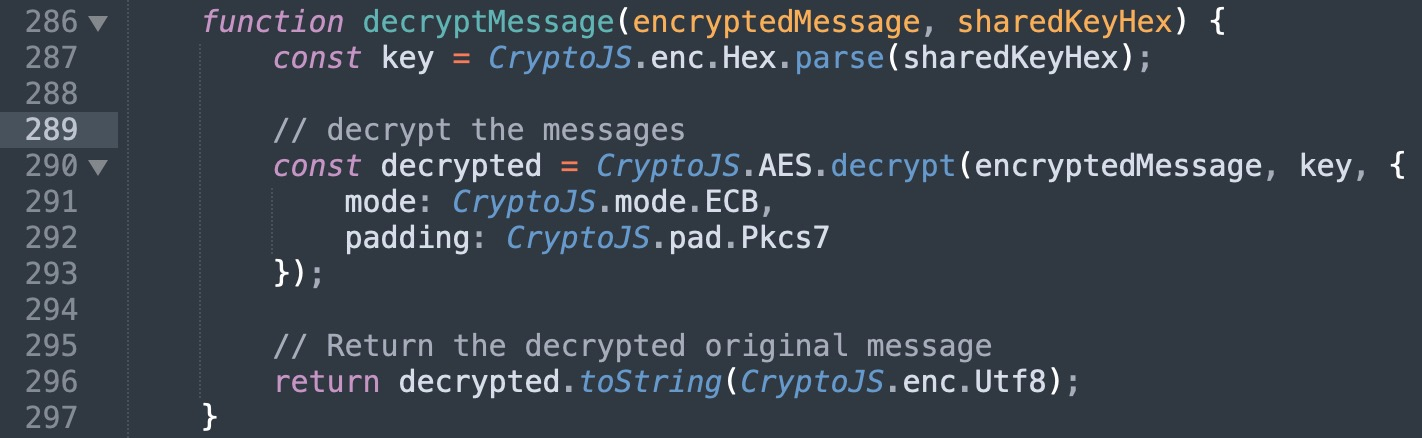
\includegraphics[width=0.8\textwidth]{graphs/decrypt_message.jpg}
                \caption{home.jinja decryptMessage \textit{line 260 - 272}}
                \label{decryptMessage}
            \end{figure}

            \begin{figure}[H]
                \centering
                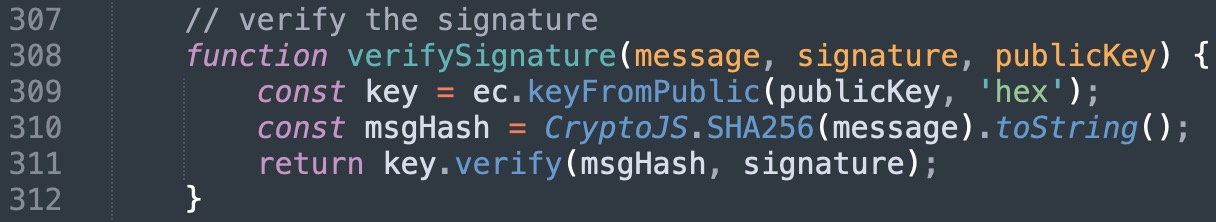
\includegraphics[width=0.8\textwidth]{graphs/verify_signature.jpg}
                \caption{home.jinja decryptMessage \textit{line 260 - 272}}
                \label{verify signature}
            \end{figure}

            \begin{figure}[H]
                \centering
                \begin{subfigure}[b]{0.75\textwidth}
                    \centering
                    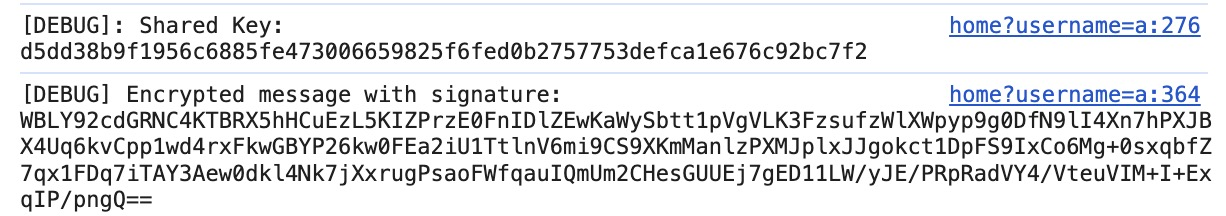
\includegraphics[width=\textwidth]{graphs/encrypt_process_sender.jpg}
                    \caption{sign and encrypt message}
                \end{subfigure}
                \hfill 
                \begin{subfigure}[b]{0.75\textwidth}
                    \centering
                    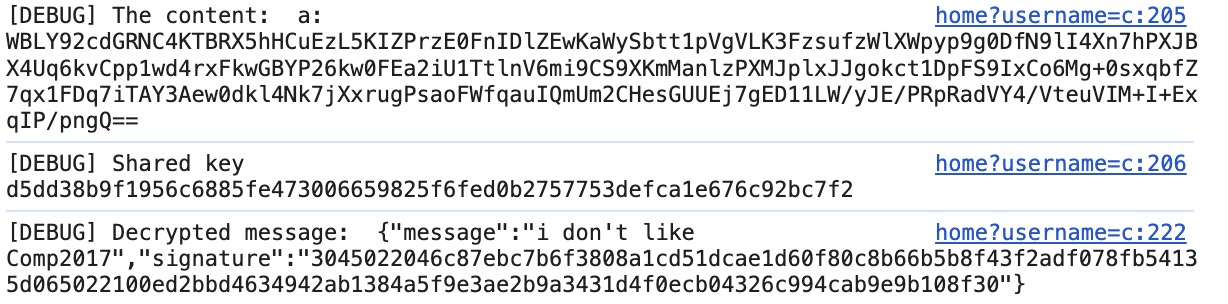
\includegraphics[width=\textwidth]{graphs/decrpt_process_receiver.jpg}
                    \caption{verify signature and decrpt message}
                \end{subfigure}
                \caption{encryption and decryption process}
                \label{encryption and decryption process}
            \end{figure}

        \item The above process combines both symmetric and asymmetric encryption and utilizes digital signatures for message authentication. Through the Diffie-Hellman key exchange \cite{gillis_diffie_hellman_2024}, we enable two users to obtain the same shared key by only exchanging public keys. This shared key is then used to encrypt messages, with the server merely acting as an intermediary. Both encryption and decryption are completed on the client side.

        \end{enumerate}

        \subsubsection*{6}
            As described in Section 5, the client sends an encrypted message to the server using a key derived from the sender's private key and the recipient's public key. The key pair is generated based on the user's password, and this process is executed on the frontend. Thus, the server never knows the shared key used for encryption/decryption, only storing the signed and encrypted messages, as shown in Figure~\ref{store history message}. Upon entering a room, users send a request to the server,as shown in figure \ref{get history message} which then retrieves the corresponding encrypted messages from the database \ref{return history message}. The frontend gets messages,computes the shared key, decrypts, and authenticates the signature, as shown in \ref{show history message}. If the verification is successful, the historical messages are displayed in the message box.

            \begin{figure}[H]
                \centering
                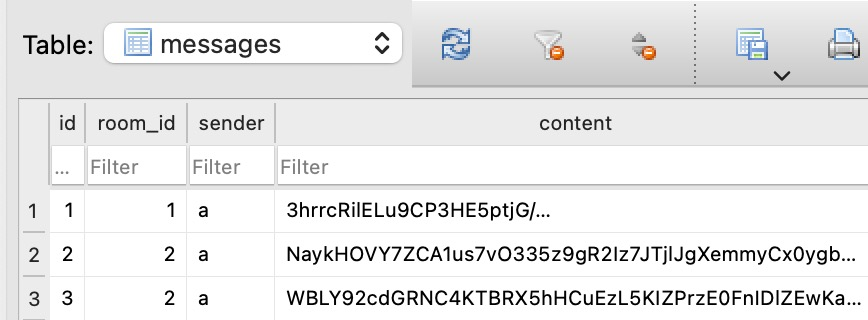
\includegraphics[width=0.8\textwidth]{graphs/store_history_message.jpg}
                \caption{main.b  \textit{Table: messages}}
                \label{store history message}
            \end{figure}

            \begin{figure}[H]
                \centering
                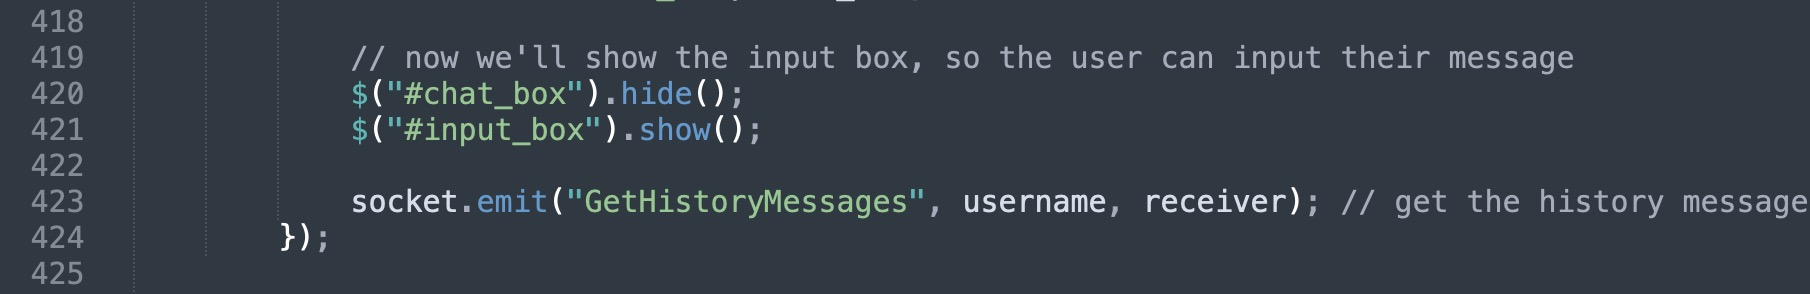
\includegraphics[width=0.8\textwidth]{graphs/join_room_get_history_message.jpg}
                \caption{\texttt{home.jinja} send a request to get history message}
                \label{get history message}
            \end{figure}

            \begin{figure}[H]
                \centering
                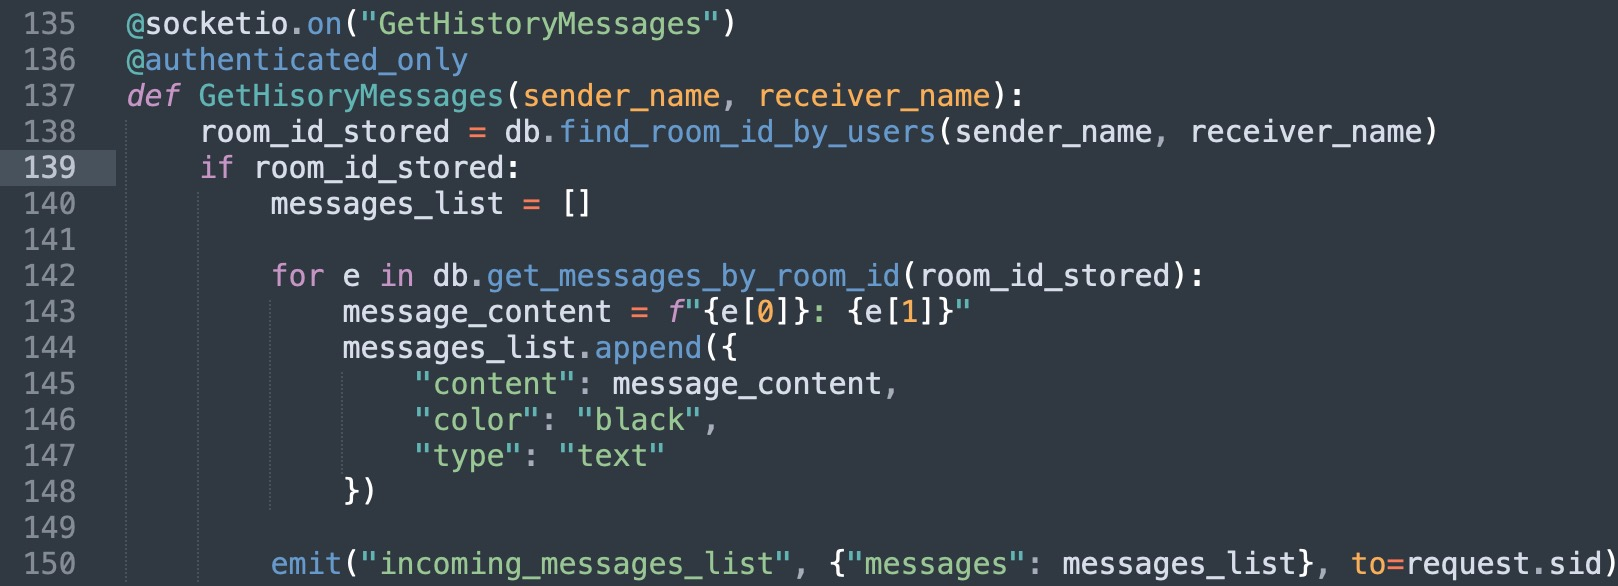
\includegraphics[width=0.8\textwidth]{graphs/return_history_message.jpg}
                \caption{\texttt{soucket\_routes.py} return history messages}
                \label{return history message}
            \end{figure}


            \begin{figure}[H]
                \centering
                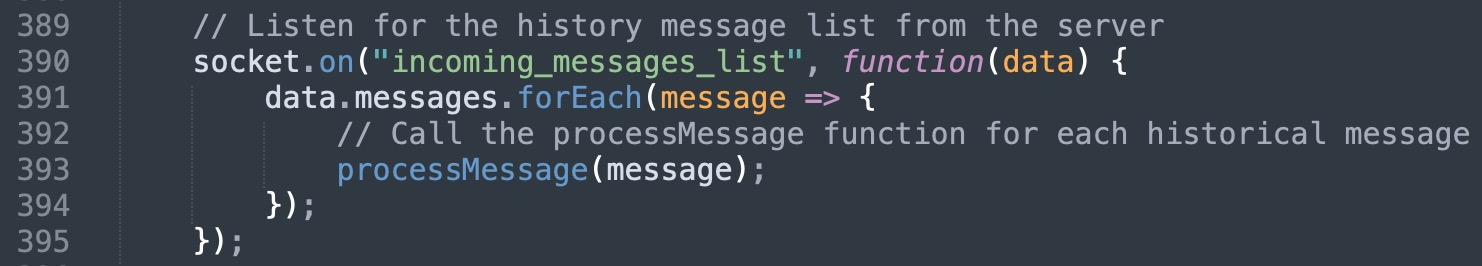
\includegraphics[width=0.8\textwidth]{graphs/show_history_message.jpg}
                \caption{\texttt{home.jinja} invoke \texttt{processMessage} to decrypt and show messages}
                \label{show history message}
            \end{figure}

    \subsection*{Part: Additional Criteria:}

        \subsubsection*{1} When signing up, after checking if the user has already signed up, the server will generate a random salt and hash the password with this salt. Finally, it stores the username, salt, and hashed password in the database.

        \begin{figure}[H]
            \centering
            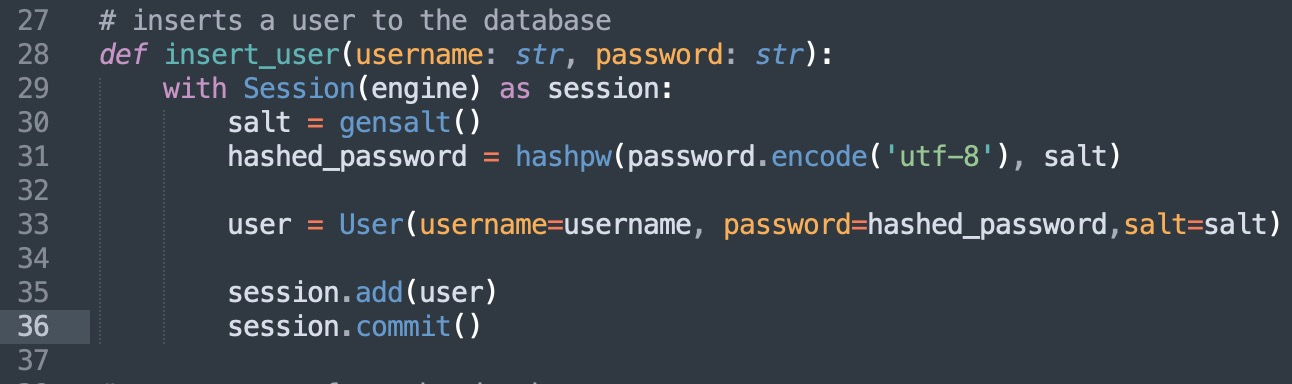
\includegraphics[width=0.8\textwidth]{graphs/insert_user.jpg}
            \caption{\texttt{db.py insert\_user()}}
        \end{figure}

        \begin{figure}[H]
            \centering
            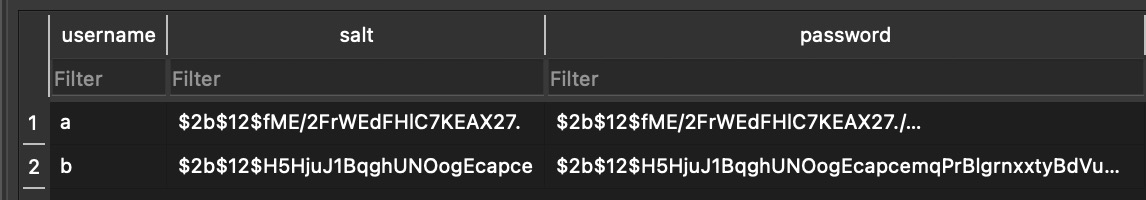
\includegraphics[width=0.8\textwidth]{graphs/hashed_passwd.jpg}
            \caption{\texttt{main.db Table: user}}
        \end{figure}

	\subsubsection*{2}Https:

        In order to implement https to make our website more secure, we first create our own SSL certificate called myCA, then we use our own SSL certificate to create a CA-signed certificate called server for our messaging website. Then we tried adding our self-created certificate to the certificate manager to make the browser trust the HTTPS encryption of the localhost. However we encountered a SAN(Subject Alternative Name) issue. To solve this problem, we used a san.cnf file to re-edit the CA-signed certificate. After updating and reinstalling it into the certificate manager, we finally achieved the https encryption for localhost(shown in Figure \ref{certificates} Figure \ref{secureconnection}). We also insures that the user can only visit our website by https(shown in Figure \ref{httpsonly}), and there won't appear any browser warnings since the website is secure and trusted by the browser.

    	\begin{figure}[H]
            \centering
            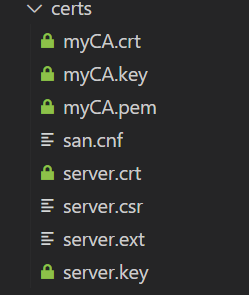
\includegraphics[width=0.2\textwidth]{zzrgraphs/certificates.png}
            \caption{all the certificates used in the project}
    		\label{certificates}
        \end{figure}

    	\begin{figure}[H]
            \centering
            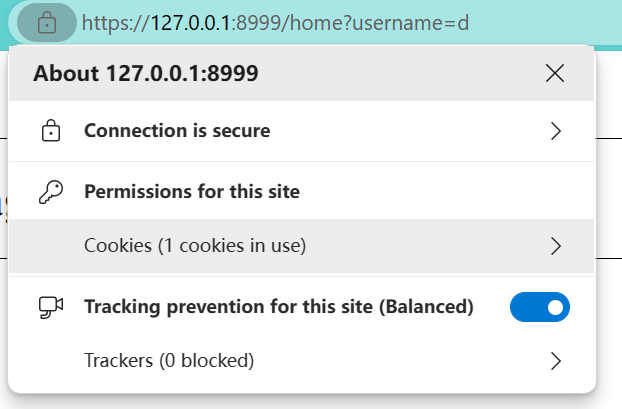
\includegraphics[width=0.4\textwidth]{zzrgraphs/connection_is_secure.png}
            \caption{the connection is secure by using https}
    		\label{secureconnection}
        \end{figure}

    	\begin{figure}[H]
            \centering
            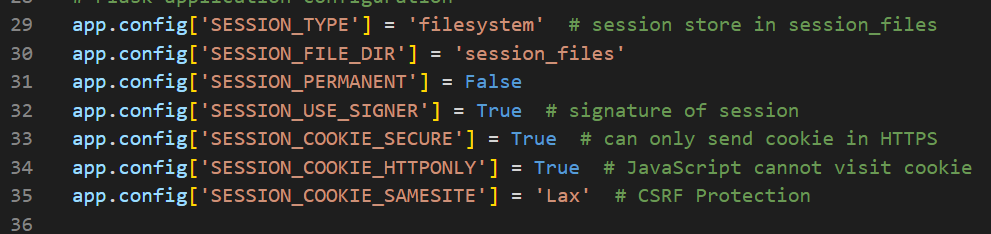
\includegraphics[width=0.8\textwidth]{zzrgraphs/cookie_secure_https_only.png}
            \caption{https only}
    		\label{httpsonly}
        \end{figure}


    \subsubsection*{3}

          By using the Flask Session library and setting a series of parameters, we have authenticated requests, as shown in the code in Figure \ref{Session setting}. Below is an explanation of the code:


        \begin{itemize}
            \item \textbf{SESSION\_TYPE = 'filesystem'}: This setting specifies that the session data will be stored on the server's file system.

            \item \textbf{SESSION\_FILE\_DIR = 'session\_files'}: This specifies the directory where session files will be stored. 

            \item \textbf{SESSION\_PERMANENT = False}: This configuration indicates that the session is not permanent, meaning the session will be cleared after the browser is closed.

            \item \textbf{SESSION\_USE\_SIGNER = True}: By enabling this, Flask will sign the session data with the application's secret key.

            \item \textbf{SESSION\_COOKIE\_SECURE = True}: This setting ensures that cookies can only be transmitted over secure (HTTPS) connections. 

            \item \textbf{SESSION\_COOKIE\_HTTPONLY = True}: This makes session cookies inaccessible to JavaScript running within the browser. 

            \item \textbf{SESSION\_COOKIE\_SAMESITE = 'Lax'}: The `SameSite` attribute of the session cookie is set to 'Lax', which helps mitigate cross-site request forgery (CSRF) attacks. 
        \end{itemize}

        \begin{figure}[H]
            \centering
            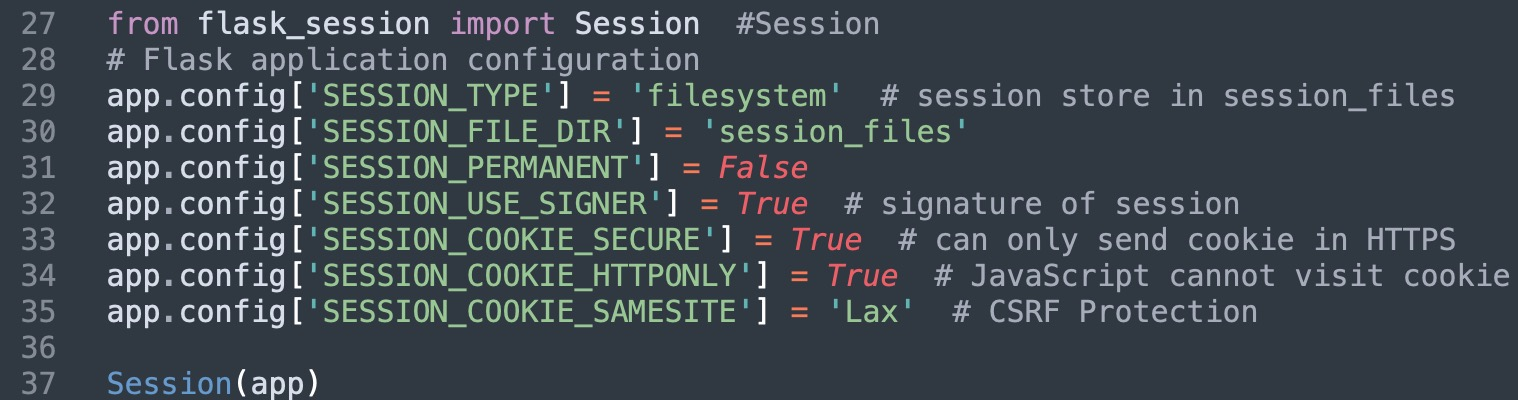
\includegraphics[width=0.8\textwidth]{graphs/session_settings.jpg}
            \caption{Session settings}
            \label{Session setting}
        \end{figure}

        In addition, we have defined the decorators \texttt{authenticated\_only} and \texttt{login\_required}, as shown in \ref{wrappers}, to verify if user sessions in the Flask application have been authenticated. These decorators are applied to functions that require a user to be logged in before execution, such as \texttt{home} in \texttt{app.py} and \texttt{connect}, \texttt{send} in \texttt{socket\_routes.py}. Moreover, in the \texttt{home} function in \texttt{app.py}, we prevent attackers from accessing data of other users by altering the URL with \texttt{username=}. This is achieved by verifying the presence of the current user in the session, as illustrated in Figures \ref{forbidden access} and \ref{home session}.

        
        \begin{figure}[H]
            \centering
            \begin{subfigure}[b]{0.75\textwidth}
                \centering
                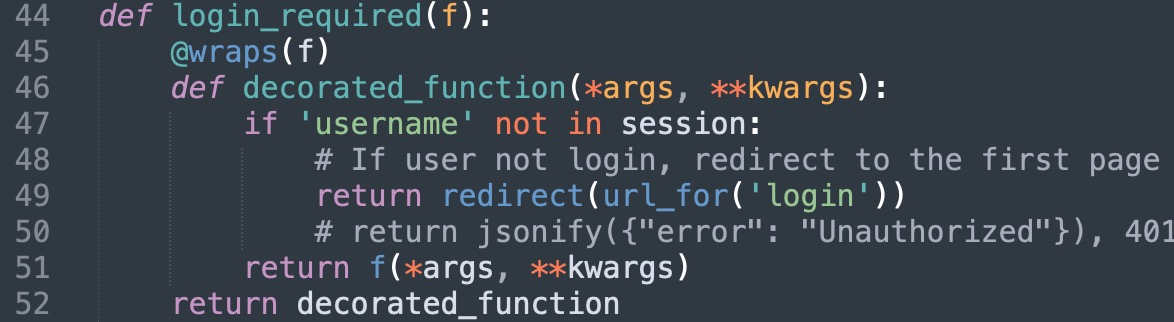
\includegraphics[width=\textwidth]{graphs/login_required.jpg}
                \caption{login\_required}
            \end{subfigure}
            \hfill 
            \begin{subfigure}[b]{0.75\textwidth}
                \centering
                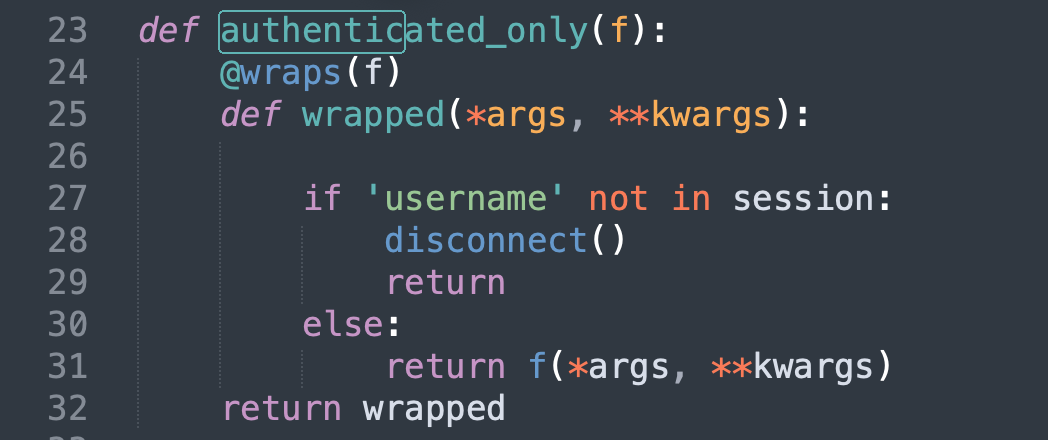
\includegraphics[width=\textwidth]{graphs/authenticated_only.jpg}
                \caption{authenticated\_only}
            \end{subfigure}
            \caption{login\_required and authenticated\_only}
            \label{wrappers}
        \end{figure}

        \begin{figure}[H]
            \centering
            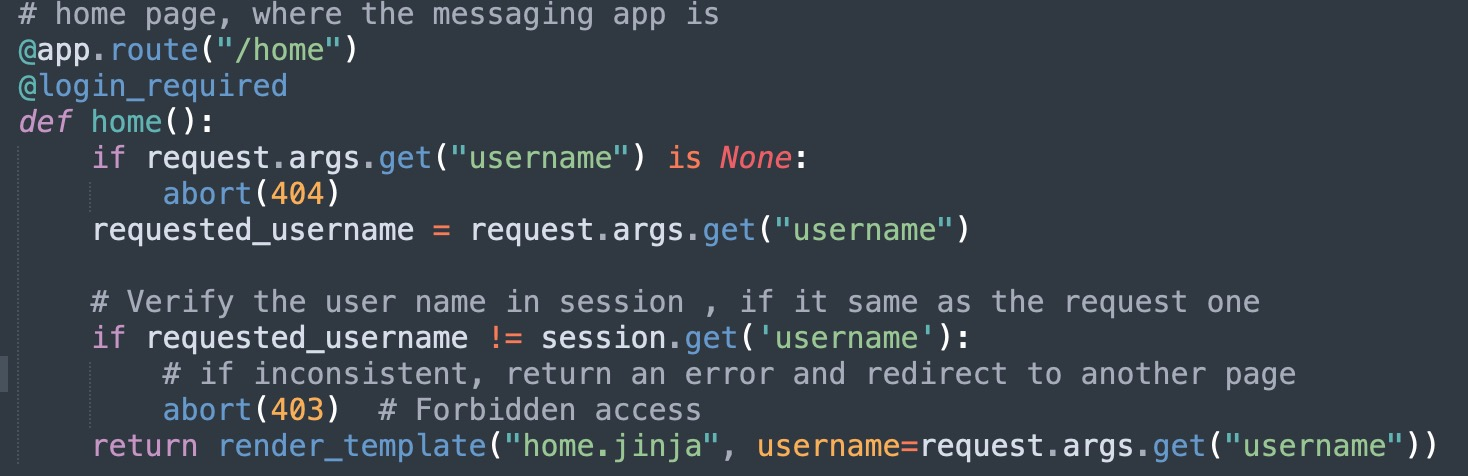
\includegraphics[width=0.8\textwidth]{graphs/forbidden_access.jpg}
            \caption{forbidden\_access}
            \label{forbidden access}{}
        \end{figure}


        \begin{figure}[H]
            \centering
            \includegraphics[width=0.8\textwidth]{graphs/home_session.jpg}
            \caption{\texttt{app.py home}}
            \label{home session}
        \end{figure}

\section{Contribution}

 Zirui Zhou:  
\begin{itemize}
\item \textbf{User login}
\item \textbf{Add friends}
\item \textbf{Friend requests}
\item \textbf{HTTPS}
\end{itemize}

\noindent Mingyuan Ba:
\begin{itemize}
\item \textbf{Chatroom}
\item \textbf{Messagehistory}
\item \textbf{Hash and salt}
\item \textbf{authentication}
\end{itemize}

Based on the Marking description on Canvas

       
\bibliographystyle{unsrt}
\bibliography{reference} 
\end{document}